\section{Synthese: Konzeption körperbasierter Interaktion im Multisensorischen Interaktionsraum}
Auf Grundlage der Analyse bestehender MIR-Szenarien wurde ein Designraum für körperbasierte Interaktion entwickelt.
Ziel dieses Kapitels ist es, aus den identifizierten Rahmenbedingungen konkrete Interaktionsanforderungen abzuleiten, mögliche Interaktionsansätze zu explorieren und schließlich ein geeignetes Interaktionsparadigma für den MIR zu konzipieren.


\subsection{Ableitung zentraler Interaktionsanforderungen}

Die Analyse der bestehenden MIR-Szenarien (vgl. Kapitel~\ref{sec:analyse}) zeigt, dass der Raum derzeit primär als immersiver Erfahrungsraum genutzt wird und nur in begrenztem Maße interaktive Steuerungsmöglichkeiten bietet. Gleichzeitig ergeben sich aus der räumlichen und technischen Gestaltung spezifische Rahmenbedingungen, die bei der Entwicklung zukünftiger Interaktionskonzepte berücksichtigt werden müssen.

Auf Grundlage dieser Beobachtungen lassen sich zentrale Anforderungen an körperbasierte Interaktionsformen im MIR ableiten.

Eine grundlegende Anforderung ergibt sich aus der Vielfalt der bestehenden Szenarien: Interaktionskonzepte sollten möglichst anwendungsübergreifend einsetzbar sein (R1). Interaktionsmechanismen sollten unabhängig von spezifischen Inhalten oder Szenariostrukturen funktionieren, um eine flexible Nutzung im gesamten System zu ermöglichen.

Darüber hinaus soll Interaktionen ohne am Körper getragene Geräte oder zusätzliche Eingabemedien möglich sein (R2). Nutzer:innen sollen ohne Controller, Maus, Tastatur oder Marker mit dem System interagieren können. Der Einsatz solcher Geräte würde einen Bruch zwischen körperlicher Präsenz im Raum und der Steuerung digitaler Inhalte erzeugen und steht damit im Widerspruch zu den in Abschnitt~\ref{sec:rw_embodied} dargestellten Prinzipien körperbasierter und realitätsnaher Interaktion.

Weiterhin soll die Interaktion die freie Bewegung der Nutzer:innen im Raum nicht einschränken (R3). Die räumliche Bewegungsfreiheit stellt eine zentrale Eigenschaft des MIR dar und trägt wesentlich zum Immersionserleben bei. Interaktionsformen sollten diese Eigenschaft unterstützen, anstatt sie durch feste Interaktionspunkte oder Gerätebindungen zu limitieren. Dies knüpft an die in Abschnitt~\ref{sec:rw_spatial} beschriebenen Zusammenhänge zwischen Raum, Körperbewegung und Interaktion an.

Zusätzlich sollte der technische Integrationsaufwand möglichst gering gehalten werden (R4). Neue Interaktionskonzepte sollten ohne umfangreiche Anpassungen bestehender Szenarien implementierbar sein und keine zusätzliche spezialisierte Hardware wie Motion-Capture-Systeme oder dedizierte Sensortechnik erfordern.

Schließlich sollte ein Interaktionssystem einen schnellen und intuitiven Zugriff auf häufig benötigte Funktionen ermöglichen, ohne die Aufmerksamkeit der Nutzer:innen dauerhaft von der immersiven Umgebung abzulenken (R5). Interaktion sollte somit unterstützend wirken, ohne die Wahrnehmung der Szene zu dominieren oder zu stören.

Die daraus abgeleiteten Anforderungen sind in Tabelle~\ref{tab:requirements} zusammengefasst.

\begin{table}[H]
\centering
\begin{tabular}{ll}
\toprule
ID & Requirement \\
\midrule
R1 & Anwendungsübergreifende Einsetzbarkeit \\
R2 & Nicht-invasive Interaktion (keine Wearables, Controller oder Marker) \\
R3 & Freie Bewegung im Raum \\
R4 & Minimaler Setupaufwand \\
R5 & Schnelle Zugriffsmöglichkeiten \\
\bottomrule
\end{tabular}
\caption{Anforderungen}
\label{tab:requirements}
\end{table}

Die Anforderungen betreffen damit sowohl die technische Integrierbarkeit als auch die Nutzbarkeit und räumliche Verträglichkeit zukünftiger Interaktionskonzepte.


\subsection{Exploration möglicher Interaktionsformen}
Auf Basis der zuvor abgeleiteten Anforderungen wurden mögliche Interaktionsformen entwickelt und systematisch hinsichtlich ihrer Eignung für den Einsatz im MIR untersucht. Ziel dieser Exploration war es, potenzielle Ansätze für körperbasierte Interaktion zu identifizieren und im Kontext der spezifischen räumlichen und technischen Gegebenheiten des Systems zu bewerten.

Die betrachteten Ansätze umfassen objekt- und sensorbezogene, kamerabasierte sowie interfacebezogene Interaktionsformen.
Dazu zählen unter anderem NFC-basierte Interaktionen mit physischen Objekten, kamerabasierte Markersysteme, UI-basierte Eingaben, gestenbasierte Interaktionen sowie positionsbasierte Steuerung durch Bewegung im Raum. Eine umfassende Übersicht der im Explorationsprozess betrachteten Möglichkeiten ist im Anhang in Abbildung~\ref{tab:interaktionsansatz} dargestellt.


Zur Strukturierung des Designraums wurden die Interaktionsansätze entlang zweier Dimensionen betrachtet: zum einen hinsichtlich ihres Explizitheitsgrades (implizit vs. explizit), zum anderen entlang grundlegender Interaktionsaufgaben räumlicher Systeme, nämlich Selektion, Manipulation und Navigation, wie sie in Abschnitt~\ref{sec:rw_spatial} eingeführt wurden.
Diese Systematisierung ermöglicht eine vergleichende Einordnung der unterschiedlichen Ansätze und unterstützt die Identifikation geeigneter Interaktionsparadigmen.

Eine vollständige Übersicht aller identifizierten Interaktionsansätze ist im Anhang dargestellt (vgl. Tab.~\ref{tab:interaktionsansatz}). Im Folgenden wird eine verdichtete Auswahl jener Ansätze präsentiert, die für die Entwicklung der nachfolgenden Konzepte als besonders relevant erachtet wurden (Tab. \ref{tab:interaktionsmoeglichkeiten}).

\begin{table}[H]
    \centering
    \small
    \caption{Verdichtete Übersicht über identifizierte Interaktionsmöglichkeiten}
    \begin{tabular}{p{0.03\linewidth} p{0.27\linewidth} >{\raggedright\arraybackslash}p{0.1\linewidth}
    >{\raggedright\arraybackslash}p{0.5\linewidth}}
        \toprule
        \textbf {Nr.} & \textbf{Interaktions\-möglichkeit} & \textbf{Art} & \textbf{Beschreibung} \\
        \midrule
        1 & Administrative Steuerung der Laut\-stärke, Helligkeit, Virbations\-inten\-sität & Explizit, Selektion & Einstellungsmöglichkeit von globaler Lautstärke, Helligkeit und Vibrationsintensität (denkbar mit Integration von lokaler Aktivierung/Deaktivierung von Licht- oder Soundquellen) \\

        2 & Präsentations\-steuerung & Explizit, Selektion & Nutzer:innen können Videomaterial abspielen, pausieren und die Wiedergabe vor-/zurückspulen \\

        3 & Objekte markieren und annotieren & Explizit, Manipulation & Nahe Inhalte oder projizierte Objekte können direkt markiert oder annotiert werden, um bestimmte Aspekte visuell zu betonen. \\

        4 & Schubbasierte Navigation & Explizit, Navigation & Eine Schubbewegung in eine bestimmte Richtung bewirkt eine Verschiebung der virtuellen Umgebung. \\

        5 & Navigation durch Gehen auf der Stelle & Explizit, Navigation & Das Gehen auf der Stelle in eine bestimmte Richtung bewirkt eine Verschiebung der virtuellen Umgebung. \\

        6 & Aktivierung von Interaktion & Explizit, Selektion & Nutzer:innen wechseln durch Annäherung oder eine initiale Geste (zum Beispiel Handheben) in einen Interaktionsmodus, um unbeabsichtigte Eingaben zu vermeiden. \\

        \bottomrule
    \end{tabular}
    \label{tab:interaktionsmoeglichkeiten}
\end{table}

Die Analyse zeigt, dass mehrere der betrachteten Ansätze nur eingeschränkt für den Einsatz im MIR geeignet sind. NFC-basierte Interaktionen eignen sich insbesondere für objektgebundene Szenarien, setzen jedoch physische Artefakte voraus und sind daher nur begrenzt universell einsetzbar. Kamerabasierte Markersysteme ermöglichen eine eindeutige Identifikation von Objekten, erfordern jedoch eine gezielte Ausrichtung auf den Kamerabereich und führen damit zu zusätzlichen Interaktionsschritten.

UI-basierte Interaktionsflächen innerhalb der Projektion bieten zwar eine klare Sichtbarkeit von Funktionen, können jedoch die immersive Wahrnehmung des Raums beeinträchtigen, da sie dauerhaft Teil der visuellen Szene sind. Gestenbasierte Interaktionen ermöglichen hingegen eine controllerlose und körpernahe Steuerung digitaler Inhalte, sind jedoch mit den in Abschnitt~\ref{sec:rw_midair} und Abschnitt~\ref{sec:rw_gestures} dargestellten Herausforderungen hinsichtlich Discoverability und Fehlinterpretation verbunden.
Positionsbasierte Interaktionen nutzen die Bewegung der Nutzer:innen im Raum als Interaktionsparameter und ermöglichen eine direkte Kopplung zwischen physischem Verhalten und Systemzustand und knüpfen damit an die in Abschnitt \ref{sec:rw_spatial} dargestellten Prinzipien räumlich eingebetteter Interaktion an.

Vor diesem Hintergrund wurden vornehmlich gestenbasierte sowie positionsbasierte Interaktionsformen als vielversprechende Ansätze identifiziert, da sie zentrale Anforderungen wie die Nutzung ohne zusätzliche Eingabegeräte sowie die Integration der räumlichen Bewegung in die Interaktion unterstützen.
Aus dem beschriebenen Designraum wurden darauf aufbauend drei Ansätze für eine vertiefte konzeptionelle Ausarbeitung ausgewählt: administrative Steuerung, objektbasierte Interaktion und positionsbasierte Navigation.
Diese Auswahl basiert darauf, dass diese Ansätze zentrale Interaktionsaufgaben in räumlichen Systemen abdecken, nämlich Selektion, Manipulation und Navigation, und zugleich unterschiedliche Grade der Explizitheit repräsentieren. Die ausgewählten Ansätze werden im Folgenden anhand exemplarischer Storyboards konkretisiert.


\subsubsection{Storyboard: Administrative Steuerung}
Das erste Storyboard zeigt ein Konzept für eine administrative Steuerung in Form eines radialen Menüs, das über eine gestenbasierte Interaktion aktiviert wird (vgl. Abb.~\ref{fig:storyboard_menu}).

Die Interaktion beginnt mit der Ausrichtung der Nutzer:innen in Richtung einer Raumwand (Abb.~\ref{fig:storyboard_menu}, a). Durch das Anheben der Hand wechselt das System in einen quasi-modalen Interaktionszustand, um die in Abschnitt~\ref{sec:rw_midair} beschriebenen Probleme unbeabsichtigter Aktivierungen in offenen Mid-Air-Interaktionsräumen zu adressieren. In diesem Zustand wird ein radial angeordnetes Menü über der Anwendung eingeblendet (Abb.~\ref{fig:storyboard_menu}, b–c). Die Wahl eines radialen Menüs knüpft an die in Abschnitt~\ref{sec:rw_menus} dargestellten Vorteile solcher Menüformen für gestenbasierte Interaktion an, insbesondere an kurze Zielwege und eine gute Sichtbarkeit verfügbarer Funktionen.

Die Auswahl von Funktionen erfolgt über die relative Position der Hand im Raum, die als Cursor innerhalb des Menüs interpretiert wird (Abb.~\ref{fig:storyboard_menu}, d). Ein kurzer Verbleib in einem Menüsegment oder eine bestätigende Geste aktiviert die jeweilige Funktion (Abb.~\ref{fig:storyboard_menu}, e-f). Zusätzlich können weitere Optionen über Untermenüs aufgerufen werden (Abb.~\ref{fig:storyboard_menu}, g). Für bestimmte Funktionen werden kontinuierliche Anpassungen ermöglicht, beispielsweise zur Steuerung von Intensitäten (Abb.~\ref{fig:storyboard_menu}, h–i). Damit greift das Storyboard die in den verwandten Arbeiten beschriebene Trennung zwischen diskreter Auswahl und weiterführender Interaktion auf.

Nach Abschluss der Interaktion wird das Menü automatisch ausgeblendet, sodass die visuelle Szene wieder in den Vordergrund tritt (Abb.~\ref{fig:storyboard_menu}, j).

Das Storyboard illustriert damit eine explizite, gestenbasierte Interaktion zur Steuerung systemweiter Funktionen und dient als konzeptionelle Grundlage für die im weiteren Verlauf detailliert ausgearbeitete Menüinteraktion.

\begin{figure}[H]
    \centering
    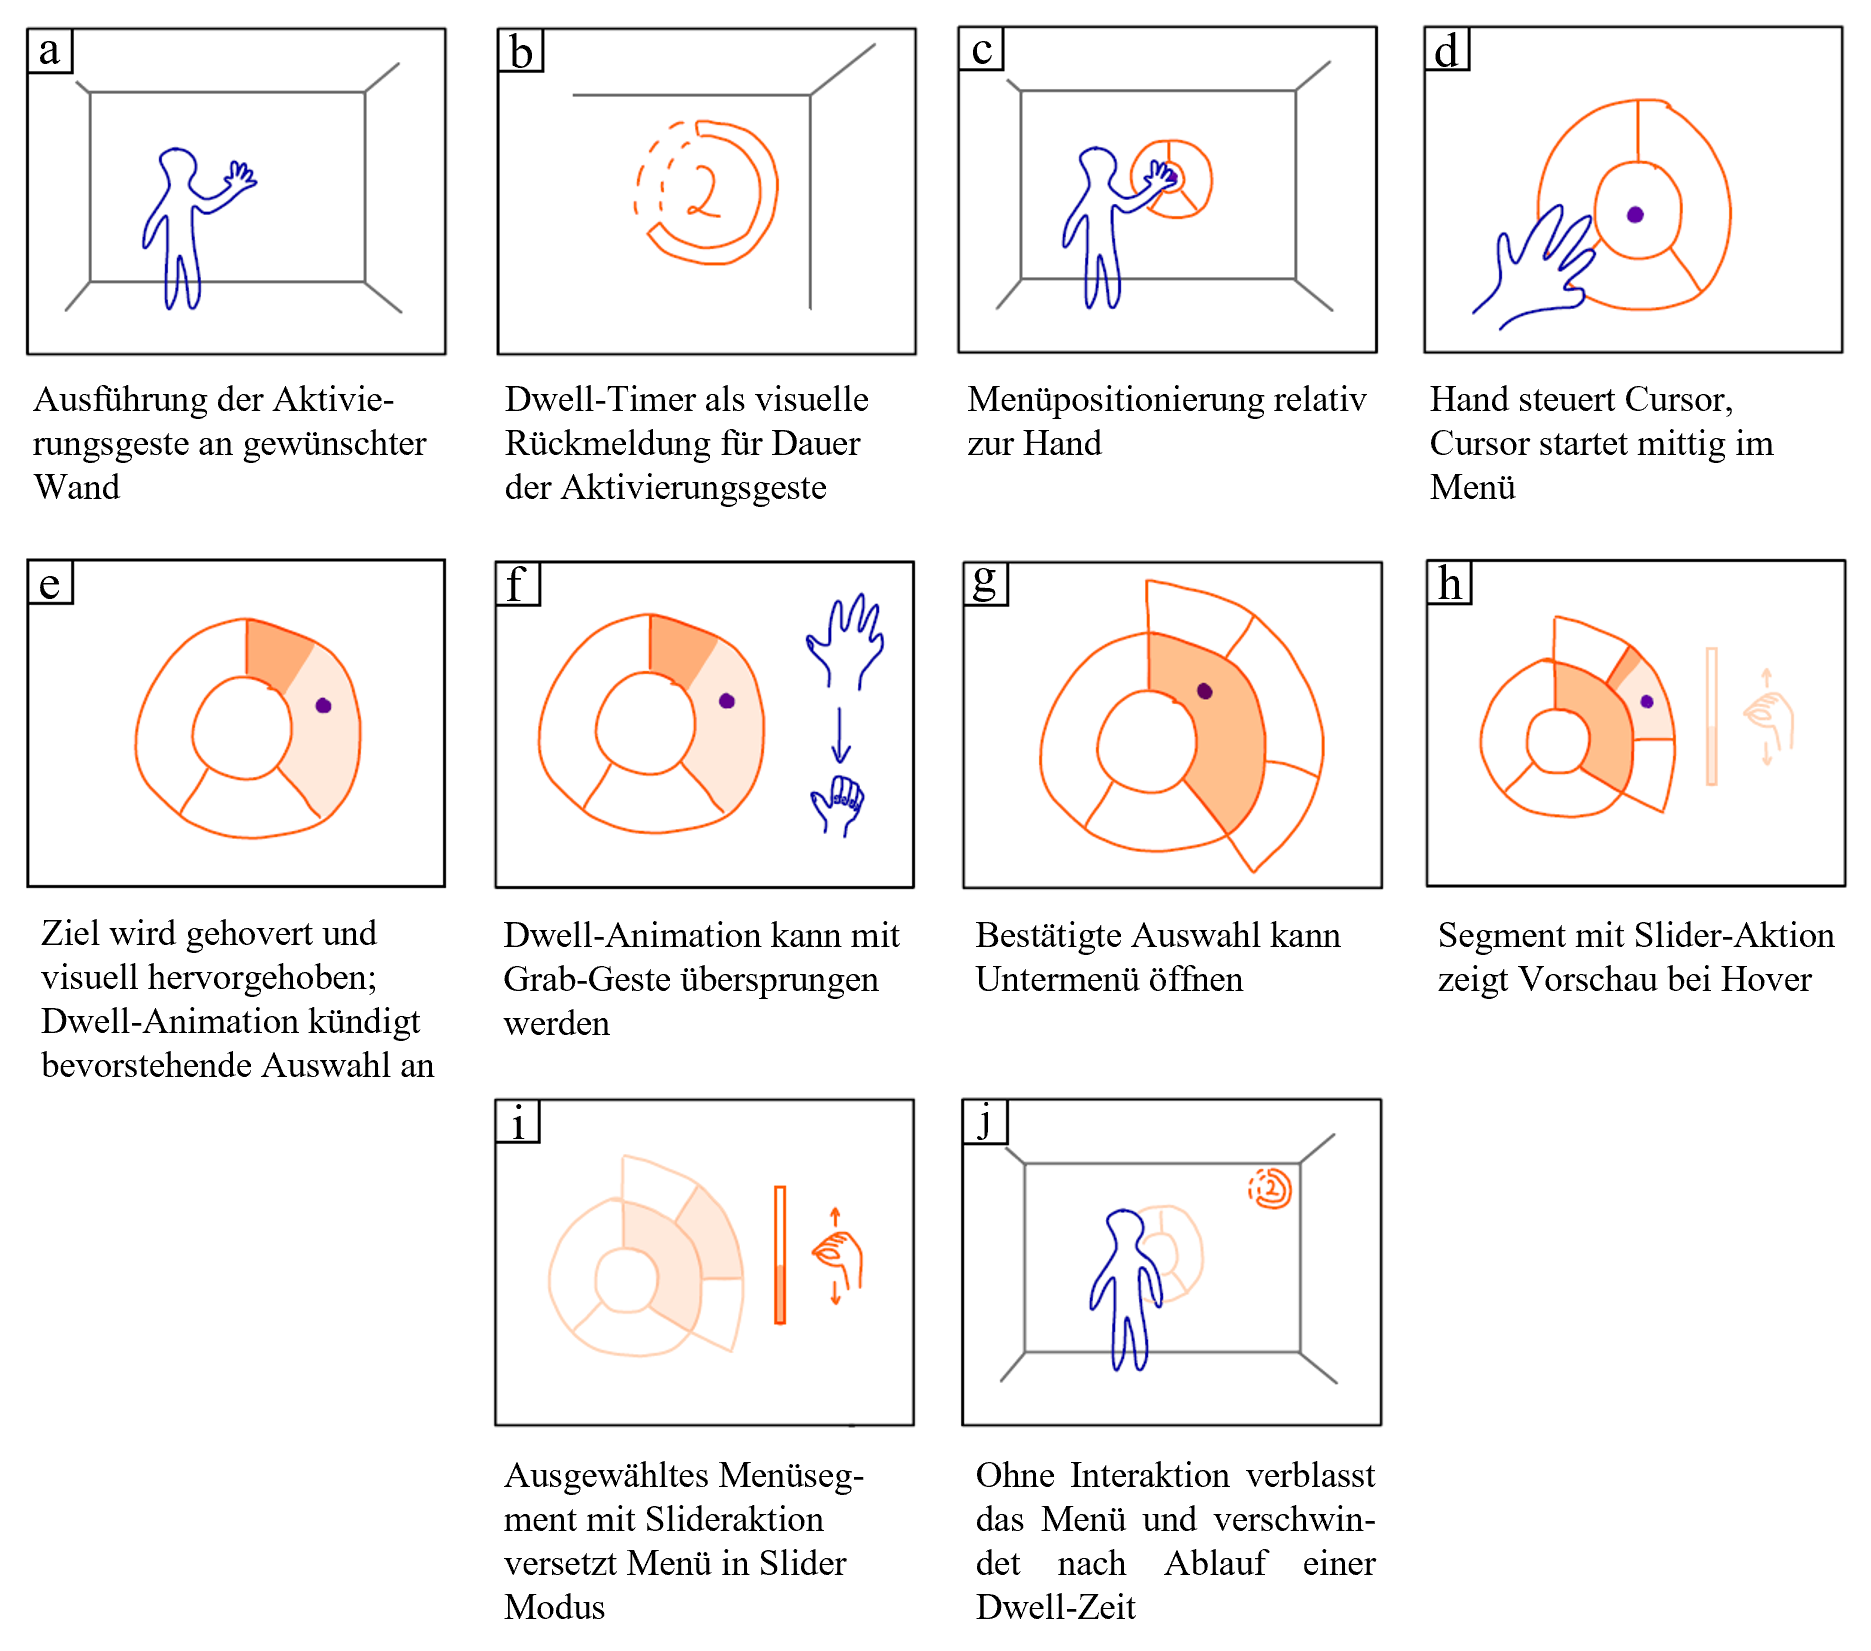
\includegraphics[width=0.98\linewidth]{content/images/storyboard_menu.png}
    \caption{Storyboard Administrative Steuerung {\color{red} Soll ich hier lieber nur 4 Pro Reihe machen, damit der Text größer ist?}}
    \label{fig:storyboard_menu}
\end{figure}


\subsubsection{Storyboard: Objektinteraktion}
Das zweite Storyboard beschreibt ein Konzept zur Objektinteraktion innerhalb der projizierten Szene.

Nach Auswahl einer Projektion positionieren sich die Nutzer:innen vor der Projektionsfläche (Abb.~\ref{fig:storyboard_paint}, a). Durch Annäherung an die Wand und das Anheben der Hand wird auch hier ein quasi-modaler Interaktionszustand aktiviert, um unbeabsichtigte Eingaben zu vermeiden und eine bewusste Interaktionsaufnahme zu ermöglichen (vgl. Abschnitt~\ref{sec:rw_midair}).

Die Handposition fungiert dabei als Cursor (Abb.~\ref{fig:storyboard_paint}, b) und überträgt ein etabliertes Interaktionsprinzip aus Desktopumgebungen in den räumlichen Kontext (vgl. \ref{sec:rw_gestures}). Dadurch bleibt die Interaktion an nachvollziehbare, körpernahe Bewegungen gekoppelt.

Gezielte Gesten ermöglichen das Setzen von Markierungen: Ein kurzer Point-and-Draw-Sweep hebt relevante Strukturen hervor (in medizinischen Szenarien beispielsweise Knochen, Muskeln oder Röntgenansichten) (Abb.~\ref{fig:storyboard_paint}, c). Dabei orientiert sich das Konzept bewusst an bekannten Handlungsmetaphern wie Zeichnen und Greifen, um eine möglichst verständliche Interaktion zu unterstützen.

Die Selektion bestehender Markierungen erfolgt über eine Grab-Geste, die das Greifen physischer Objekte imitiert. Durch Halten der Geste können Markierungen entfernt werden (Abb.~\ref{fig:storyboard_paint}, d–e).

Das Konzept adressiert damit zentrale Interaktionsaufgaben räumlicher Systeme, insbesondere Selektion und Manipulation, wie sie in Abschnitt \ref{sec:rw_spatial} eingeführt wurden, und dient als Grundlage für die weitere Ausgestaltung inhaltsbezogener Interaktionen im MIR.

\begin{figure}[H]
    \centering
    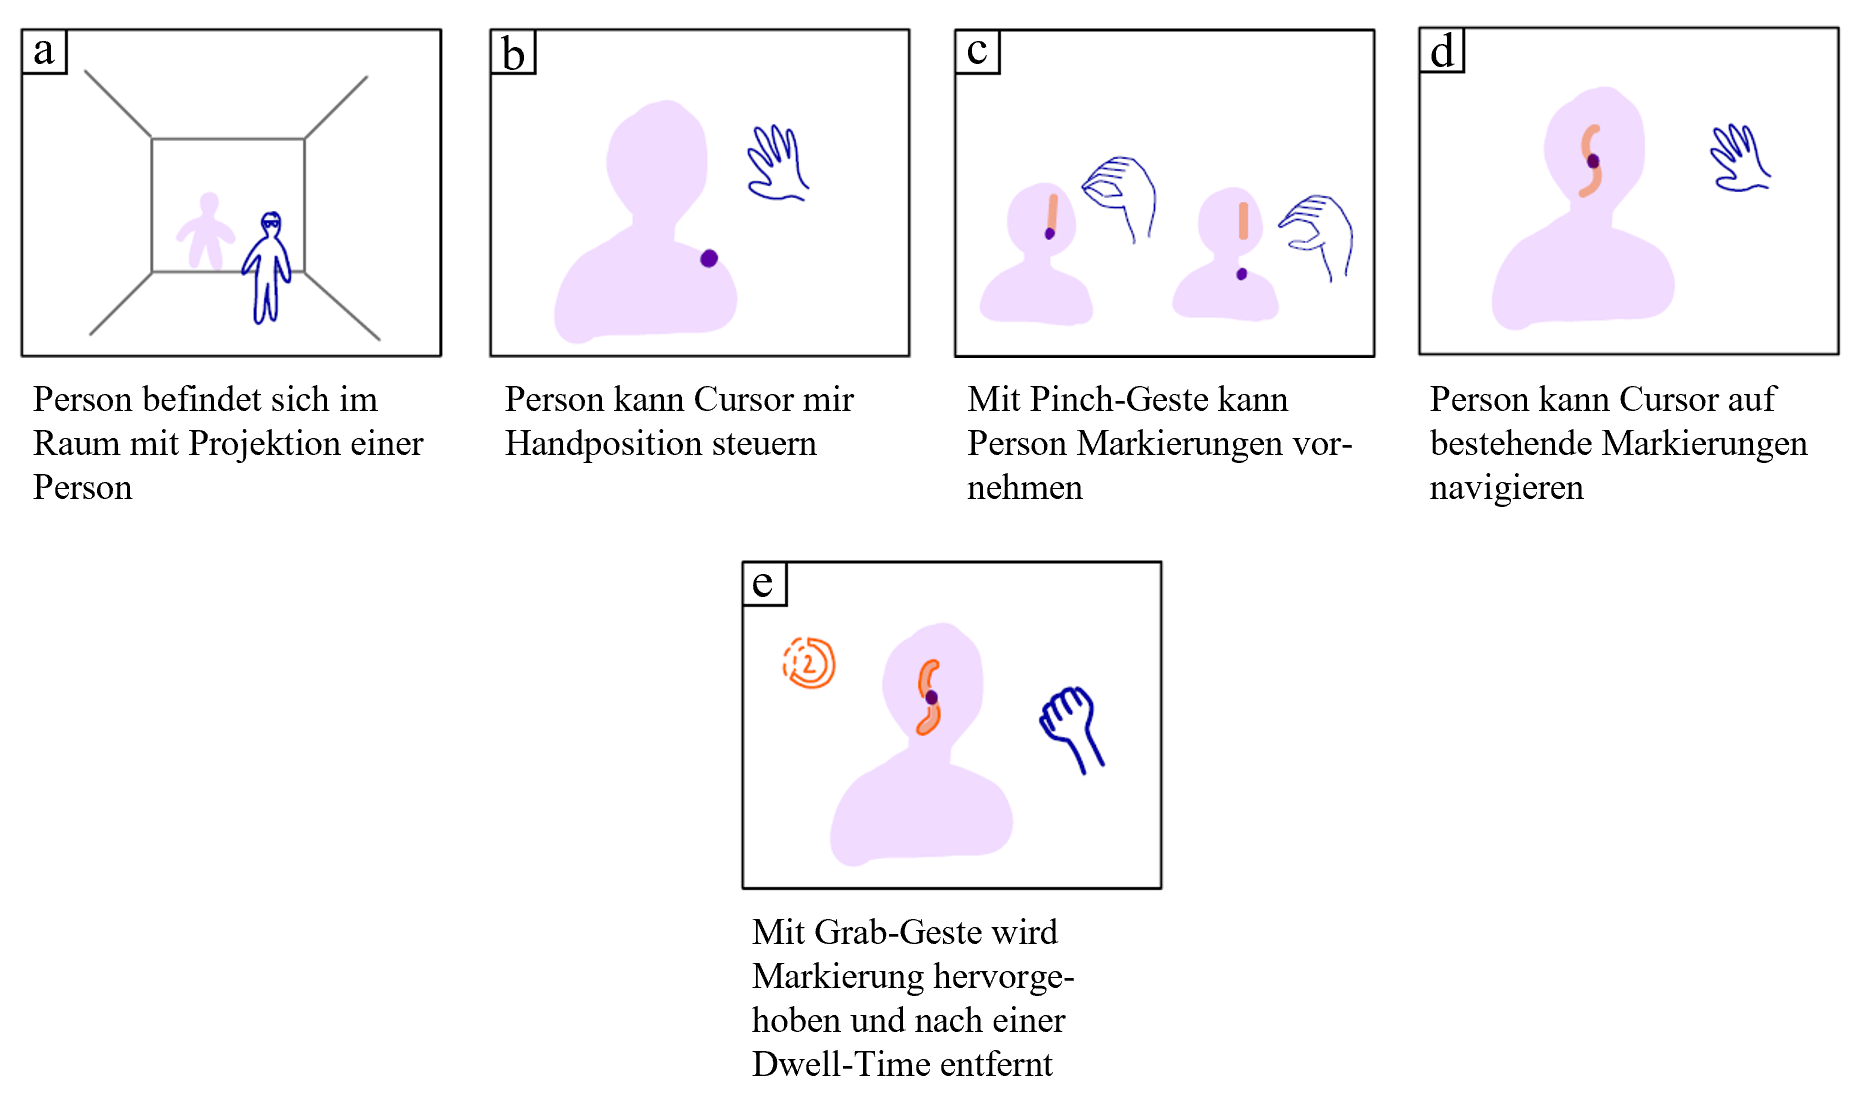
\includegraphics[width=0.98\linewidth]{content/images/storyboard_paint.png}
    \caption{Storyboard Objektinteraktion}
    \label{fig:storyboard_paint}
\end{figure}


\subsubsection{Storyboard: Navigation im Raum}
Das dritte Storyboard (Abb. \ref{fig:storyboard_navigation}) skizziert zwei Konzepte für positionsbasierte Navigation, die die körperliche Bewegung der Nutzer:innen als primären Interaktionsparameter nutzen, um eine Fortbewegung in der virtuellen Szene ohne zusätzliche Eingabegeräte zu ermöglichen.

Der erste Ansatz basiert auf einer schubbasierten Navigation (Abb. \ref{fig:storyboard_navigation}, a-c), die als steering-based Methode klassifiziert werden kann (vgl. \ref{sec:rw_navigation}). Hierbei bewegen sich Nutzer:innen in die gewünschte Richtung und initiieren die Fortbewegung durch eine aktive Schubbewegung mit den Händen. Diese explizite Kopplung von Position, Geste und virtueller Bewegung ermöglicht eine hohe Kontrolle und kann als besonders immersive Interaktionsform gelten, da Körperbewegung und virtuelle Fortbewegung eng aufeinander bezogen sind (vgl. Abschnitt~\ref{sec:rw_navigation})

% TODO FIX Satz
Der zweite Ansatz nutzt Walking-in-Place (vgl. \ref{sec:rw_navigation}), also das Gehen auf der Stelle als Auslöser virtueller Fortbewegung. Auch hier richten sich die Nutzer:innen zunächst in die Richtung aus, in die navigiert werden soll (Abb. \ref{fig:storyboard_navigation}, d-e). Die Bewegung wird durch eine Laufgeste auf der Stelle eingeleitet und aktiviert nach einer kurzen Verweildauer die Navigation im Raum (Abb. \ref{fig:storyboard_navigation}, f), welche durch die Bewegung der Szene in die entsprechende Richtung eine kontinuierliche Fortbewegung simuliert (Abb. \ref{fig:storyboard_navigation}, g). Die Bewegung endet, sobald die Nutzer:innen ihre Position verändern oder Walking-in-Place stoppen. Diese Methode ist besonders für physisch begrenzte Räume wie den MIR geeignet, da sie die kognitiven Vorteile natürlicher Fortbewegung simuliert, ohne ein großes Platzangebot vorauszusetzen.

Beide Ansätze verfolgen das Ziel, Navigation ohne zusätzliche Eingabegeräte zu ermöglichen und die körperliche Bewegung im Raum als primären Interaktionsparameter zu nutzen. Während die schubbasierte Variante eine aktive und bewusst gesteuerte Interaktion darstellt,
etzt die Walking-in-Place-Variante auf eine reduzierte zusätzliche Gestik und eine stärker bewegungsbasierte Steuerung.

Das Storyboard illustriert damit unterschiedliche Ausprägungen positionsbasierter Navigation und dient als Grundlage für die weitere Auswahl und Ausarbeitung geeigneter Interaktionskonzepte im MIR.

\begin{figure}[H]
    \centering
    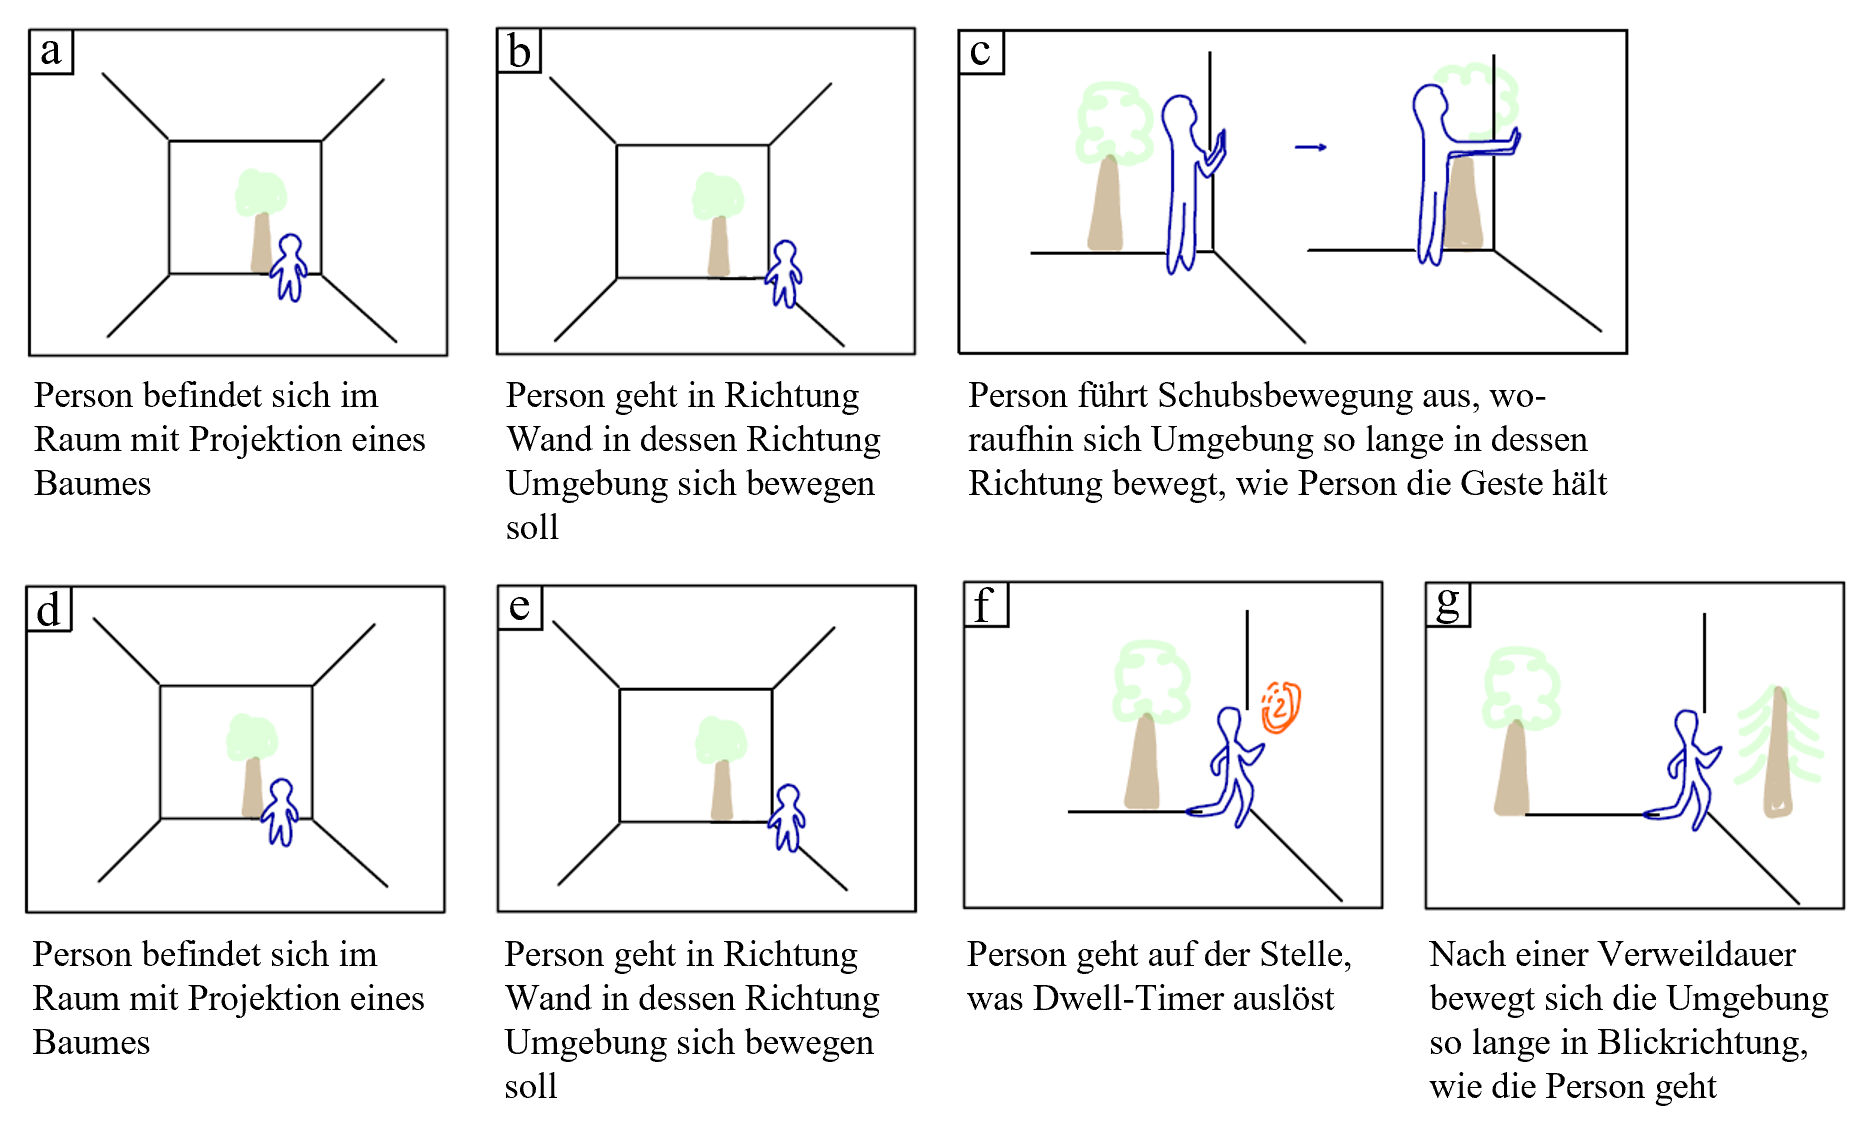
\includegraphics[width=0.98\linewidth]{content/images/storyboard_navigation.png}
    \caption{Storyboard für Navigation im Raum}
    \label{fig:storyboard_navigation}
\end{figure}


\subsection{Auswahl eines geeigneten Interaktionsparadigmas}
%Obwohl das Öffnen des Menüs eine temporäre Unterbrechung der atmosphärischen Erfahrung darstellt, ermöglicht es eine strukturierte, konsistente und lernbare Interaktion. Die Nutzer:innen können sich auf die Auswahl konzentrieren, ohne sich für jede Einstellung eine eigene Geste merken zu müssen. Die Unterbrechung ist kurz, aber notwendig, um die Komplexität der multisensorischen Steuerung zu reduzieren.


%Die Kombination aus diskreter Auswahl über das Marking Menu und kontinuierlicher Anpassung über einen Slider stellt einen sinnvollen Kompromiss dar. Während die Auswahl über das Menü strukturiert und lernbar ist, ermöglicht der Slider eine feine, kontinuierliche Anpassung – ohne dass Nutzer:innen für jede Einstellung eine eigene Geste erlernen müssen. Dies reduziert die kognitive Belastung und erhöht die Effizienz, ohne die Immersion vollständig zu unterbrechen.

Die im Rahmen der konzeptionellen Exploration entwickelten Storyboards repräsentieren drei grundlegende Interaktionsansätze im MIR: administrative Steuerung über ein Menü, objektbasierte Interaktion innerhalb der Szene sowie positionsbasierte Navigation im Raum. 

Diese drei Ansätze unterscheiden sich hinsichtlich ihrer Übertragbarkeit auf bestehende MIR-Szenarien. Die positionsbasierte Navigation setzt voraus, dass Bewegung im Raum selbst Teil der Anwendung ist, etwa im Sinne freier Fortbewegung innerhalb einer virtuellen Umgebung. Wie die Analyse der bestehenden MIR-Szenarien gezeigt hat (Abschnitt \ref{sec:analyse}), ist dies derzeit jedoch nur im Dschungel-Szenario vertreten. Für die überwiegend vorgerenderten Anwendungsszenarien ist dieser Ansatz daher nur eingeschränkt geeignet.

Auch objektbasierte Interaktionen sind nur limitiert generalisierbar. Sie setzen explizite Interaktionsobjekte oder markierbare Inhalte innerhalb der Szene voraus und erfordern damit eine entsprechende Gestaltung oder Anpassung der jeweiligen Anwendung. Da viele der bestehenden MIR-Szenarien keine solchen Interaktionspunkte vorsehen, ist dieser Ansatz nur eingeschränkt auf das Gesamtsystem übertragbar.

Im Gegensatz dazu ist eine administrative Steuerung über ein Menü unabhängig von der konkreten Szenariostruktur einsetzbar. Sie ermöglicht den Zugriff auf systemweite Funktionen, ohne dass die zugrunde liegenden Anwendungen angepasst werden müssen, und weist damit eine hohe Generalisierbarkeit auf. Beispielsweise sind allgemeine Einstellungen wie Lautstärke, Helligkeit und Vibrationsintensität in den meisten Szenarien relevant und unabhängig von deren konkreter Struktur zugänglich.
Sie ermöglichen eine controllerlose Bedienung und lassen sich direkt an natürliche Handbewegungen der Nutzer:innen koppeln. Damit unterstützen sie zentrale Anforderungen wie die Nutzung ohne zusätzliche Eingabegeräte (R2) sowie die Erhaltung der Bewegungsfreiheit im Raum (R3). Diese Einschätzung deckt sich mit den in Abschnitt \ref{sec:rw} dargestellten Potenzialen körperbasierter und Mid-Air-basierter Interaktion (vgl. Abschnitt~\ref{sec:rw_embodied} und Abschnitt~\ref{sec:rw_midair}).

Gleichzeitig stellt die Gestaltung geeigneter Interaktionsmechanismen im dreidimensionalen Raum eine Herausforderung dar.
Abschnitt~\ref{sec:rw_midair} und Abschnitt~\ref{sec:rw_menus} zeigen, dass klassische grafische Benutzungsschnittstellen nur eingeschränkt auf Mid-Air-Interaktionen übertragbar sind, da sie in der Regel für zweidimensionale Displays und präzise Eingabegeräte optimiert wurden.

Komplexe gestenbasierte Interaktionssysteme wurden im Rahmen dieser Arbeit jedoch bewusst nicht als primärer Interaktionsmechanismus gewählt. Obwohl Gesten eine natürliche Form körperbasierter Interaktion darstellen, weisen solche Systeme mehrere Herausforderungen auf. Wie in den verwandten Arbeiten dargestellt, gehen freie Gestensysteme häufig mit einer geringen Discoverability, einer erhöhten Lernanforderung sowie dem Risiko unbeabsichtigter Aktivierungen einher (vgl. Abschnitt~\ref{sec:rw_midair} und Abschnitt~\ref{sec:rw_gestures}). Darüber hinaus können Gestenerkennungssysteme in offenen Interaktionsräumen zu Fehlinterpretationen führen, wenn alltägliche Bewegungen fälschlicherweise als Interaktion interpretiert werden.

Um diese Herausforderungen zu adressieren, wurde ein menübasiertes Interaktionskonzept gewählt, das verfügbare Funktionen explizit sichtbar macht und gleichzeitig eine gestenbasierte Steuerung ermöglicht. Wie in Abschnitt~\ref{sec:rw_menus} gezeigt, eignen sich Marking-Menus besonders für solche Kontexte, da sie kurze Zielwege, eine hohe Erlernbarkeit und die Unterstützung motorischen Lernens kombinieren.
Vor diesem Hintergrund wurden Marking-Menus als zentrales Interaktionsparadigma für den MIR ausgewählt.


\subsection{Konzeption des Interaktionssystems} % Hauptkapitel + hier nochmal Requirements erwähnen?
\label{sec:synthese_konzeption_des_interaktionssystems}


% ZUSAMMENGEFASST MIT QUELLEN:

% Bei der Auswahl eines Schiebereglers tritt das Menü visuell zurück, um den Fokus zu lenken. Eine Pinch-Geste, die an die Nutzung physischer Regler erinnert, wird durch ein Icon eingeführt, um von bekannten Metaphern zu profitieren \parencite{LaViola20043DUserInterfaces, jacob2008realitybasedinteraction}.


Auf Basis der getroffenen Auswahl wird das Konzept einer menübasierten, gestenbasierten Interaktion im Folgenden weiter konkretisiert. Während das Storyboard bereits die grundlegende Interaktionsidee und den Nutzungskontext skizziert, liegt der Fokus dieses Kapitels auf der detaillierten Ausgestaltung des Interaktionsmechanismus.

Dabei werden zentrale Designentscheidungen hinsichtlich Struktur, Interaktionsablauf und visueller Gestaltung des radialen Menüs hergeleitet. \\

Das entwickelte Interaktionskonzept kombiniert kamerabasiertes Handtracking mit einem radialen Menü, das als zentrale Interaktionsschnittstelle zwischen Nutzer:innen und Zielanwendung fungiert. Die Position der Hand im Raum wird dabei als Cursor interpretiert, über den Nutzer:innen mit dem Menü interagieren können. Das Menü wird als Overlay über der jeweiligen Zielanwendung eingeblendet und ermöglicht den Zugriff auf systemweite Steuerungsfunktionen, ohne dass die bestehende Anwendung angepasst werden muss.

Durch diese Entkopplung von Interaktion und Anwendung wird eine flexible und szenariounabhängige Nutzung des Systems ermöglicht.


\subsubsection{Handtracking und Cursor}
\label{sec:synthese_handtracking}

Die Position der Hand im Raum wird als primärer Interaktionspunkt genutzt und dient als Cursor innerhalb des Overlays. Die Interpretation der Handposition orientiert sich bewusst an bekannten Interaktionsmustern aus etablierten Benutzungsoberflächen und überträgt diese in den räumlichen Kontext. Die Nutzung dieses Prinzips soll dazu beitragen, dass Nutzer:innen das System und die Steuerungsmöglichkeiten ohne vorherige Anleitung anwenden können (vgl. Abschnitt~\ref{sec:rw_gestures} zu Evolutionary Gestures).

Im Gegensatz zu klassischen Eingabegeräten wie Maus oder Controller entsteht dadurch eine direkte räumliche Beziehung zwischen Nutzerbewegung und Systemreaktion. Gleichzeitig können Nutzer:innen ihre Hände frei im Raum bewegen, wodurch die Interaktion mit der natürlichen Bewegungsfreiheit im MIR vereinbar bleibt (R3). \\

{\color{red} Ist es störend, dass ich hier von der Menüpositionierung spreche? Aber eigentlich ist es ja wichtig um zu verstehen, wieso die Cursorposition so gewählt wird + als Kontext für den Interaktionsraum}
Das Menü und der Cursor werden standardmäßig nicht angezeigt, sondern muss durch Nutzer:innen mit einer Aktivierungsgeste (vgl. Abbildung \ref{fig:openpalm_gesture_image_no_marking}) erst aktiviert werden. Dies verhindert die versehentliche Auslösung der Menüinteraktion (vgl. Abschnitt~\ref{sec:rw_midair}), sodass die Immersion der Zielanwendung nicht unbeabsichtigt unterbrochen wird. Nach erfolgreicher Aktivierung wird das Menü an einer festen Position im Raum eingeblendet, standardmäßig in der Mitte des aktiven Bildschirms. Der Cursor wird jedoch initial im Zentrum positioniert, sodass die Interaktion relativ zu diesem Ausgangspunkt erfolgt. Dadurch entsteht ein lokaler Interaktionsraum um die Aktivierungsposition herum (vgl. Abb.~\ref{fig:Interaktionsraum}), der unabhängig von der Körpergröße oder Haltung der Nutzer:innen genutzt werden kann. Diese Gestaltung ermöglicht eine konsistente und ergonomische Interaktion, da Nutzer:innen das Menü aus unterschiedlichen Positionen im Raum heraus aktivieren können, ohne dass die relative Erreichbarkeit der Menüelemente beeinflusst wird. Zugleich adressiert sie die in Abschnitt~\ref{sec:rw_midair}  beschriebenen Ermüdungsprobleme länger gehaltener Mid-Air-Interaktion, da Nutzer:innen selbst bestimmen können, in welcher Haltung die Interaktion am komfortabelsten für sie ist.

\begin{figure}[H]
    \centering
    \begin{subfigure}{0.27\textwidth}
        \centering
        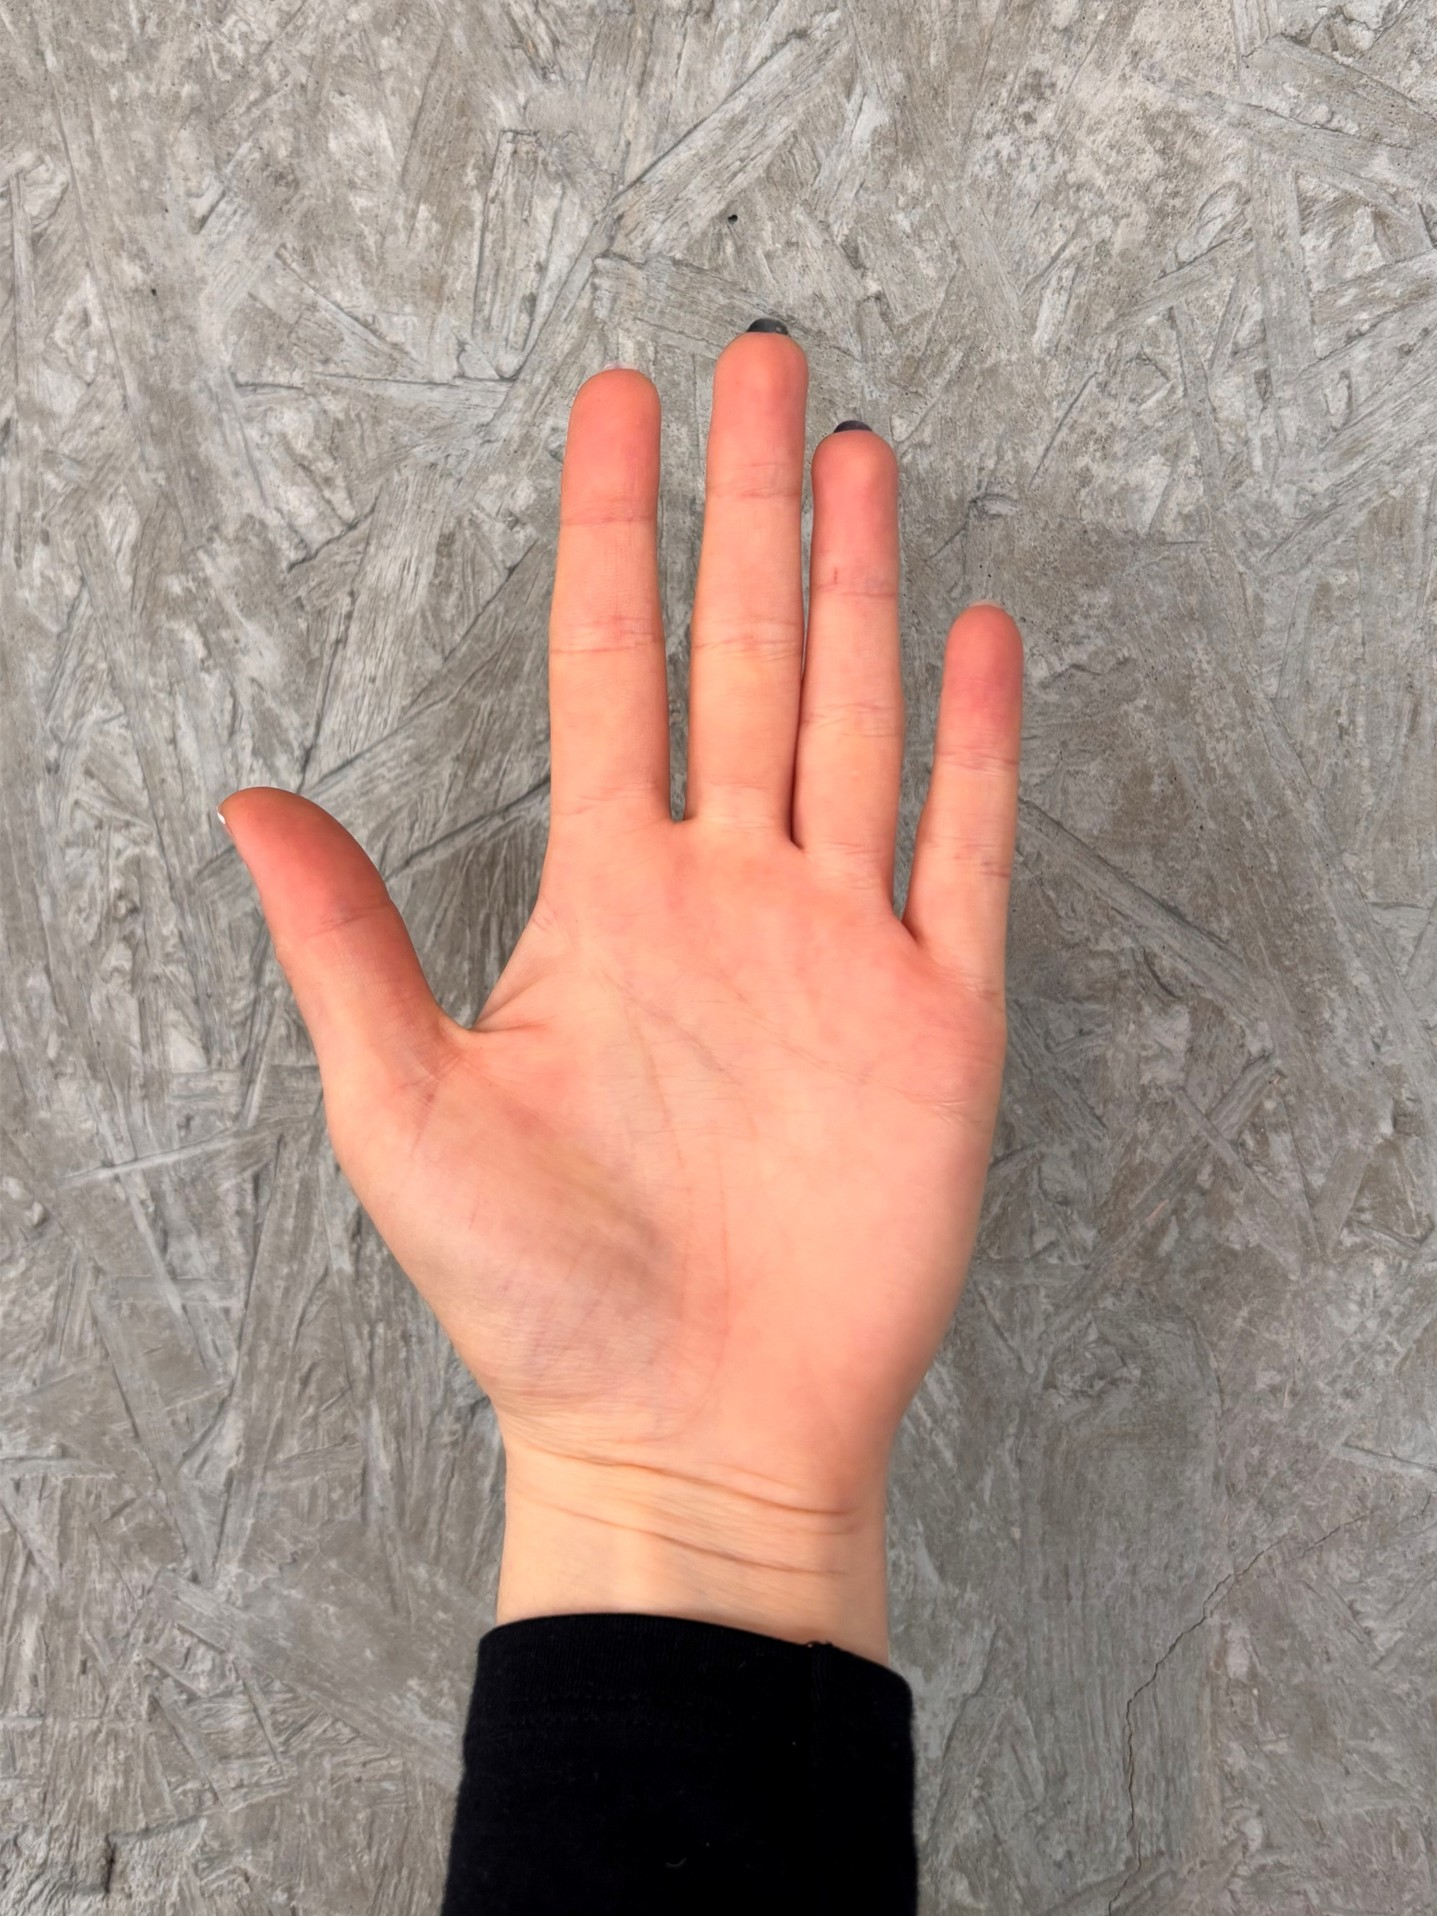
\includegraphics[
            width=\linewidth
        ]{content/images/open_palm.jpg}
        \caption{Aktivierungsgeste}
        \label{fig:openpalm_gesture_image_no_marking}
    \end{subfigure}
    \hspace{0.5cm}
    \begin{subfigure}{0.65\textwidth}
        \centering
        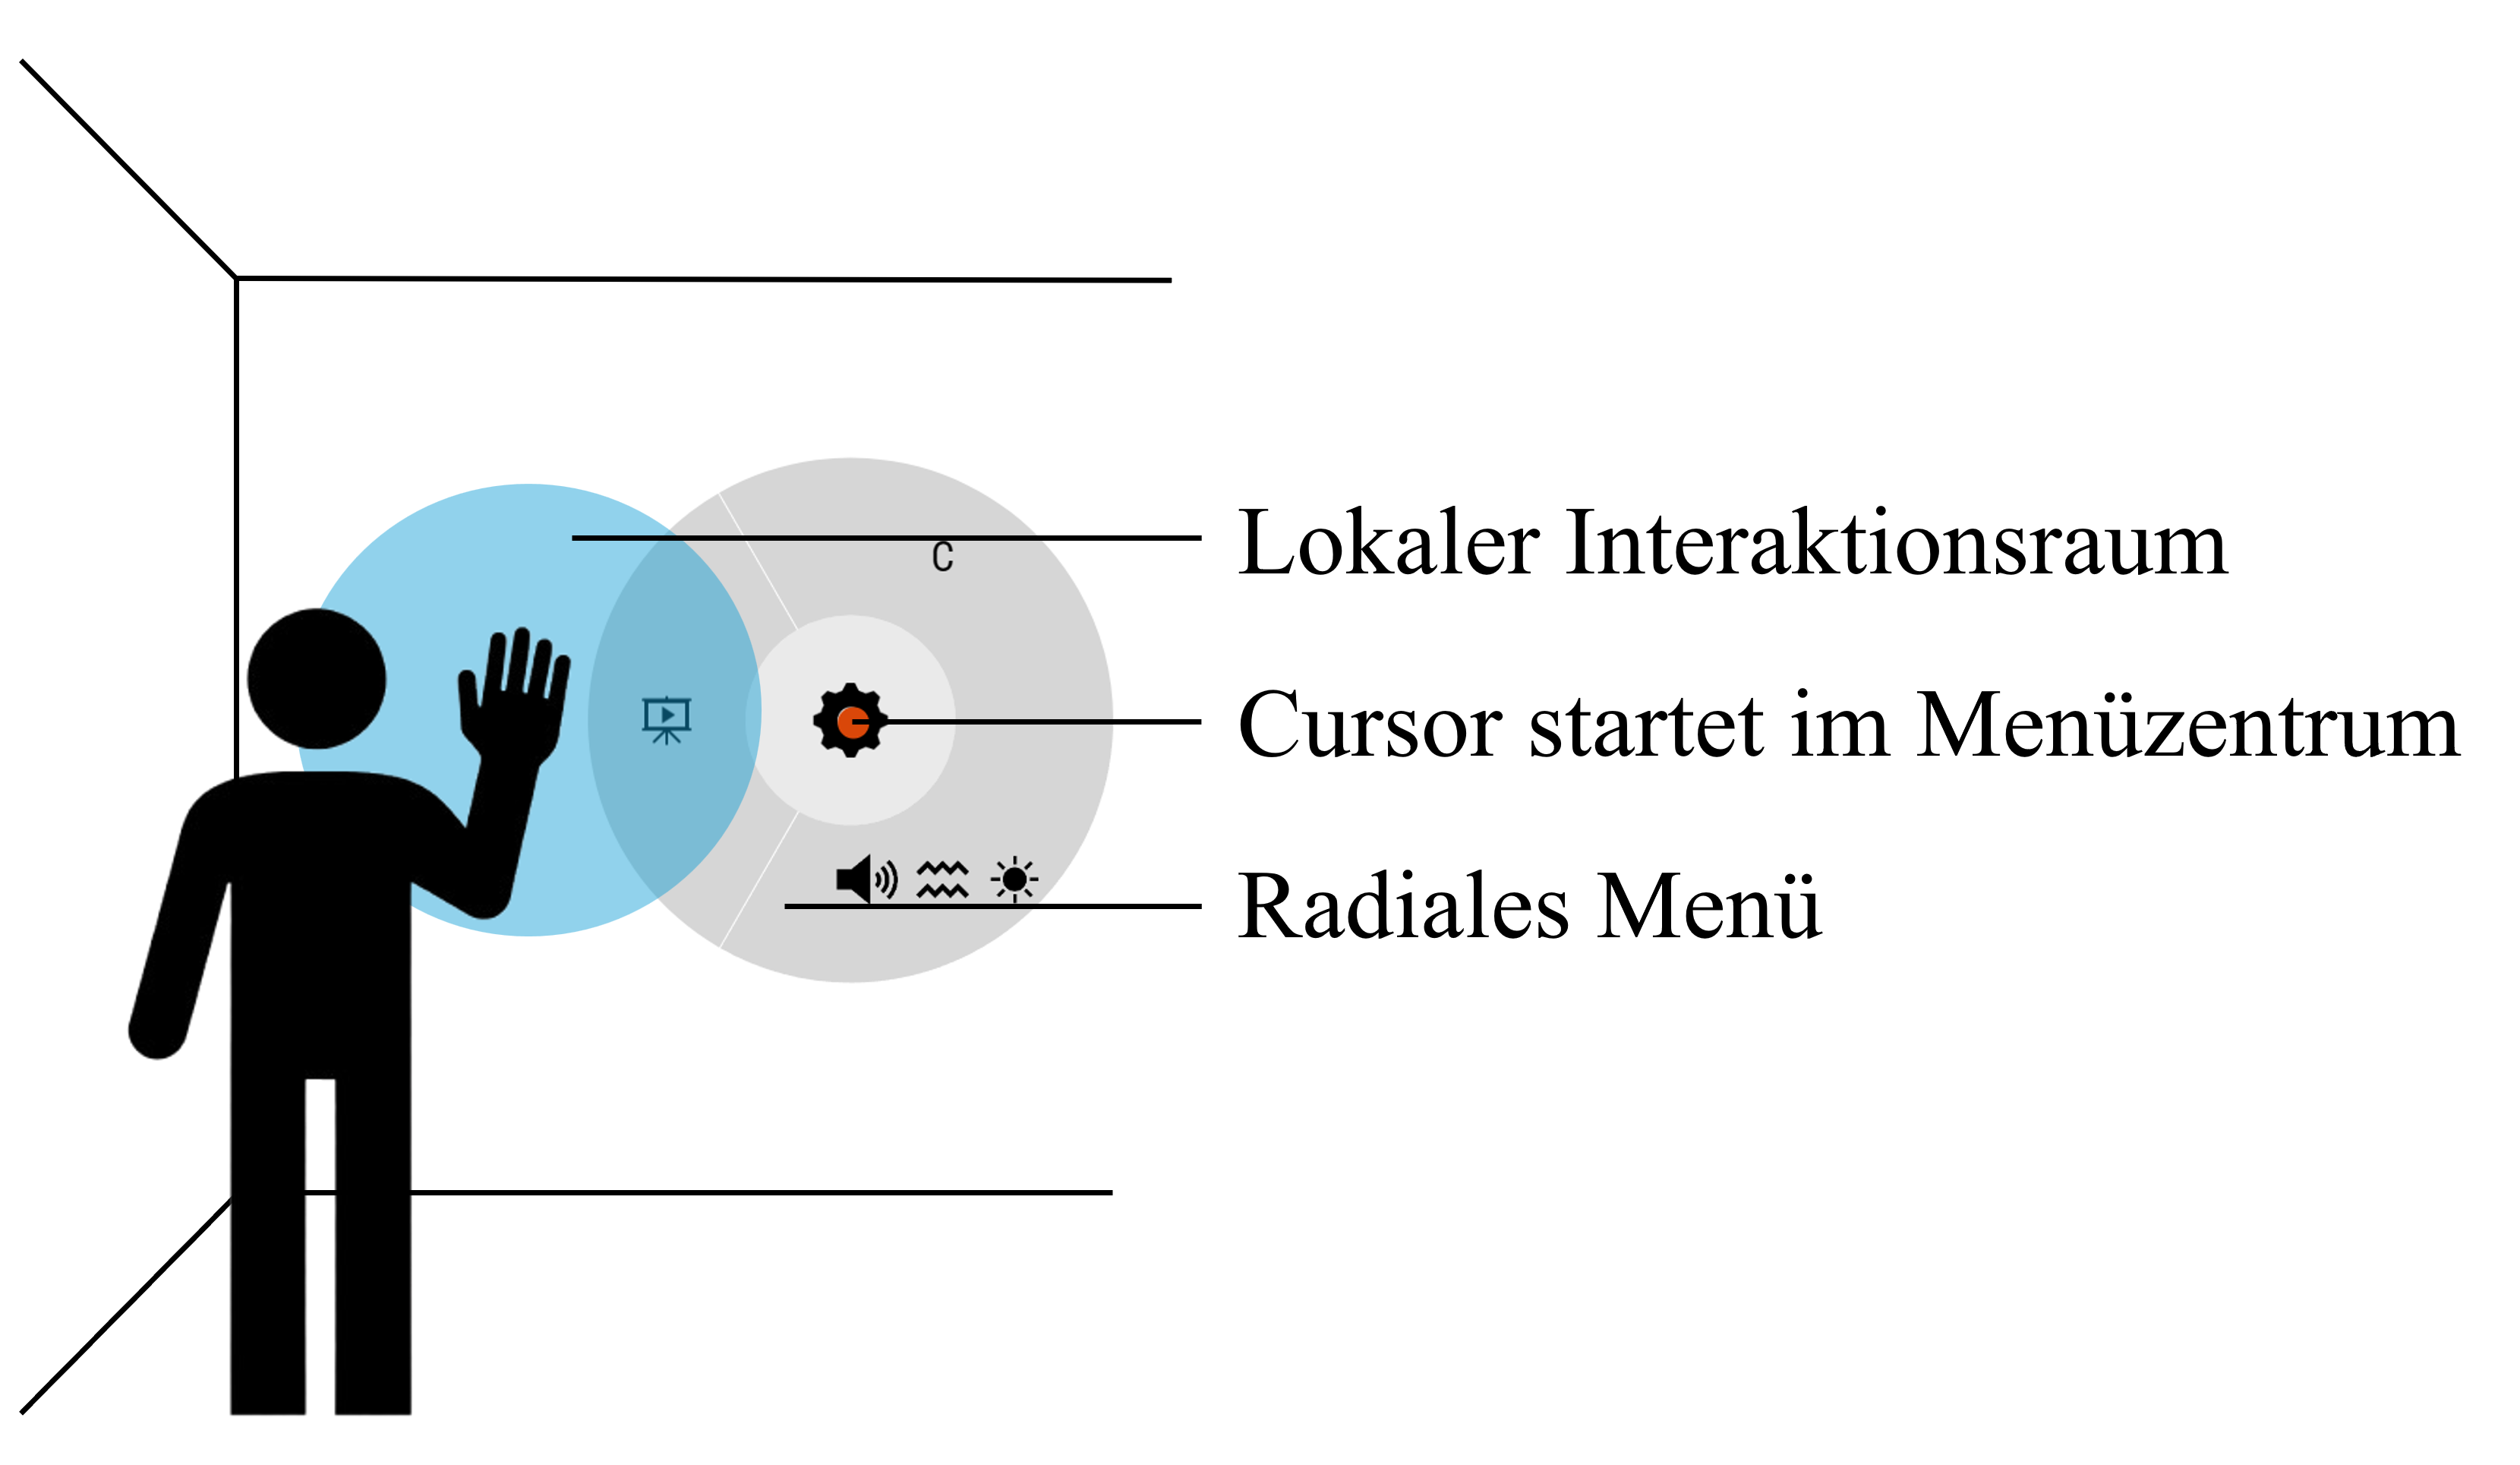
\includegraphics[
            width=\linewidth
        ]{content/images/Interaktionsraum.png}
        \caption{Schematische Darstellung des Interaktionsraums}
        \label{fig:interaktionsraum}
    \end{subfigure}
    \caption{Darstellung der Aktivierungsgeste und des lokalen Interaktionsraums}
    \label{fig:interaction_start}
\end{figure}

Zur weiteren Vereinfachung der Interaktion wird nicht zwischen linker und rechter Hand unterschieden. Dadurch wird die Komplexität reduziert und die Bedienbarkeit erhöht, da Nutzer:innen beliebig die Interaktionshand wechseln können.

Die Hand fungiert somit als zentraler Interaktionsanker, über den Auswahl- und Steuerungsaktionen ausgeführt werden können. Dadurch kann auf zusätzliche Eingabegeräte verzichtet werden, während gleichzeitig eine natürliche und intuitive Interaktion ermöglicht wird.


\subsubsection{Radiales Menü}
\label{sec:synthese_radiales_menü}
Als zentrale Interaktionsschnittstelle wurde ein Marking-Menu als gestanbasierte Variante eines radialen Menüs gewählt. Diese Entscheidung knüpft an die in Abschnitt~\ref{sec:rw_menus} dargestellten Vorteile dieser Menüform für Mid-Air-Interaktion an, insbesondere an kurze Zielwege, gleichmäßige Erreichbarkeit und die Unterstützung motorischen Lernens.

{\color{red} TODO: Hier könnte auch abschnitt über Menüpositionierung rein - eher hier oder in Handtracking (?) - meine tendenz handtracking}

Vor dem Hintergrund der in Abschnitt~\ref{sec:rw_menus} diskutierten Zusammenhänge zwischen Menütiefe, Segmentbreite und Präzision wird eine moderate Anzahl an Einträgen pro Ebene angestrebt, jedoch nicht erzwungen. Eine hohe Anzahl von Segmenten führt dazu, dass die einzelnen Einträge zunehmend kleiner werden. Dadurch verringert sich nicht nur die Interaktionsfläche für den Cursor, sondern auch der verfügbare Platz für Beschriftungen der Menüsegmente. Aus diesem Grund wurde entschieden, Icons anstelle textueller Labels zu verwenden.

Da im MIR nicht die möglichst schnelle Ausführung von Aufgaben im Vordergrund steht, sondern eine intuitive, verständliche und in den Raum eingebettete Interaktion, und die konkrete Menüstruktur maßgeblich durch die jeweilige Zielanwendung bestimmt wird, ist eine starre Begrenzung der Segmentanzahl jedoch nicht in allen Fällen zielführend. Stattdessen erscheint es sinnvoll, bei der Gestaltung auf potenzielle Usability-Probleme hinzuweisen, die sich insbesondere aus großer Menütiefe oder vielen Einträgen ergeben können.


\subsubsection{Auswahlmechanismen}
Für die Auswahl von Menüeinträgen wurden zwei unterschiedliche Interaktionsmechanismen vorgesehen: eine aktive Greifgeste sowie eine zeitbasierte Auswahl (Dwell Selection). Diese Kombination greift die in Abschnitt~\ref{sec:rw_gestures} dargestellten Vor- und Nachteile impliziter und expliziter Selektionsmechanismen auf.

Die Dwell-basierte Auswahl ermöglicht einen niedrigschwelligen Zugriff auf Menüfunktionen, da sie keine zusätzliche Bestätigungsgeste voraussetzt. Damit eignet sie sich insbesondere für Erstnutzende oder für Situationen, in denen möglichst wenig gestische Komplexität erforderlich ist. Gleichzeitig ist, wie in Abschnitt~\ref{sec:rw_gestures} diskutiert, bekannt, dass Dwell-basierte Verfahren leicht verständlich sein können, jedoch mit längeren Interaktionszeiten einhergehen können.

Zusätzlich wurde eine Greifgeste als explizite Auswahlmethode vorgesehen (Abb. \ref{fig:grab_gesture}). Dabei orientiert sich das Konzept bewusst an einer vertrauten Handlungsmetapher des Greifens und somit physichen Auswählens, um die Erlernbarkeit zu unterstützen. Um die Discoverability der expliziten Geste zu fördern, wird sie durch einen visuellen Hinweis eingeführt (Abb. \ref{fig:grab_hint}). Dies adressiert die in Abschnitt~\ref{sec:rw_gestures} diskutierte Bedeutung von Guessability und Discoverability in gestenbasierten Systemen.

\begin{figure}[H]
    \centering
    \begin{subfigure}[t]{0.27\textwidth}
        \centering
        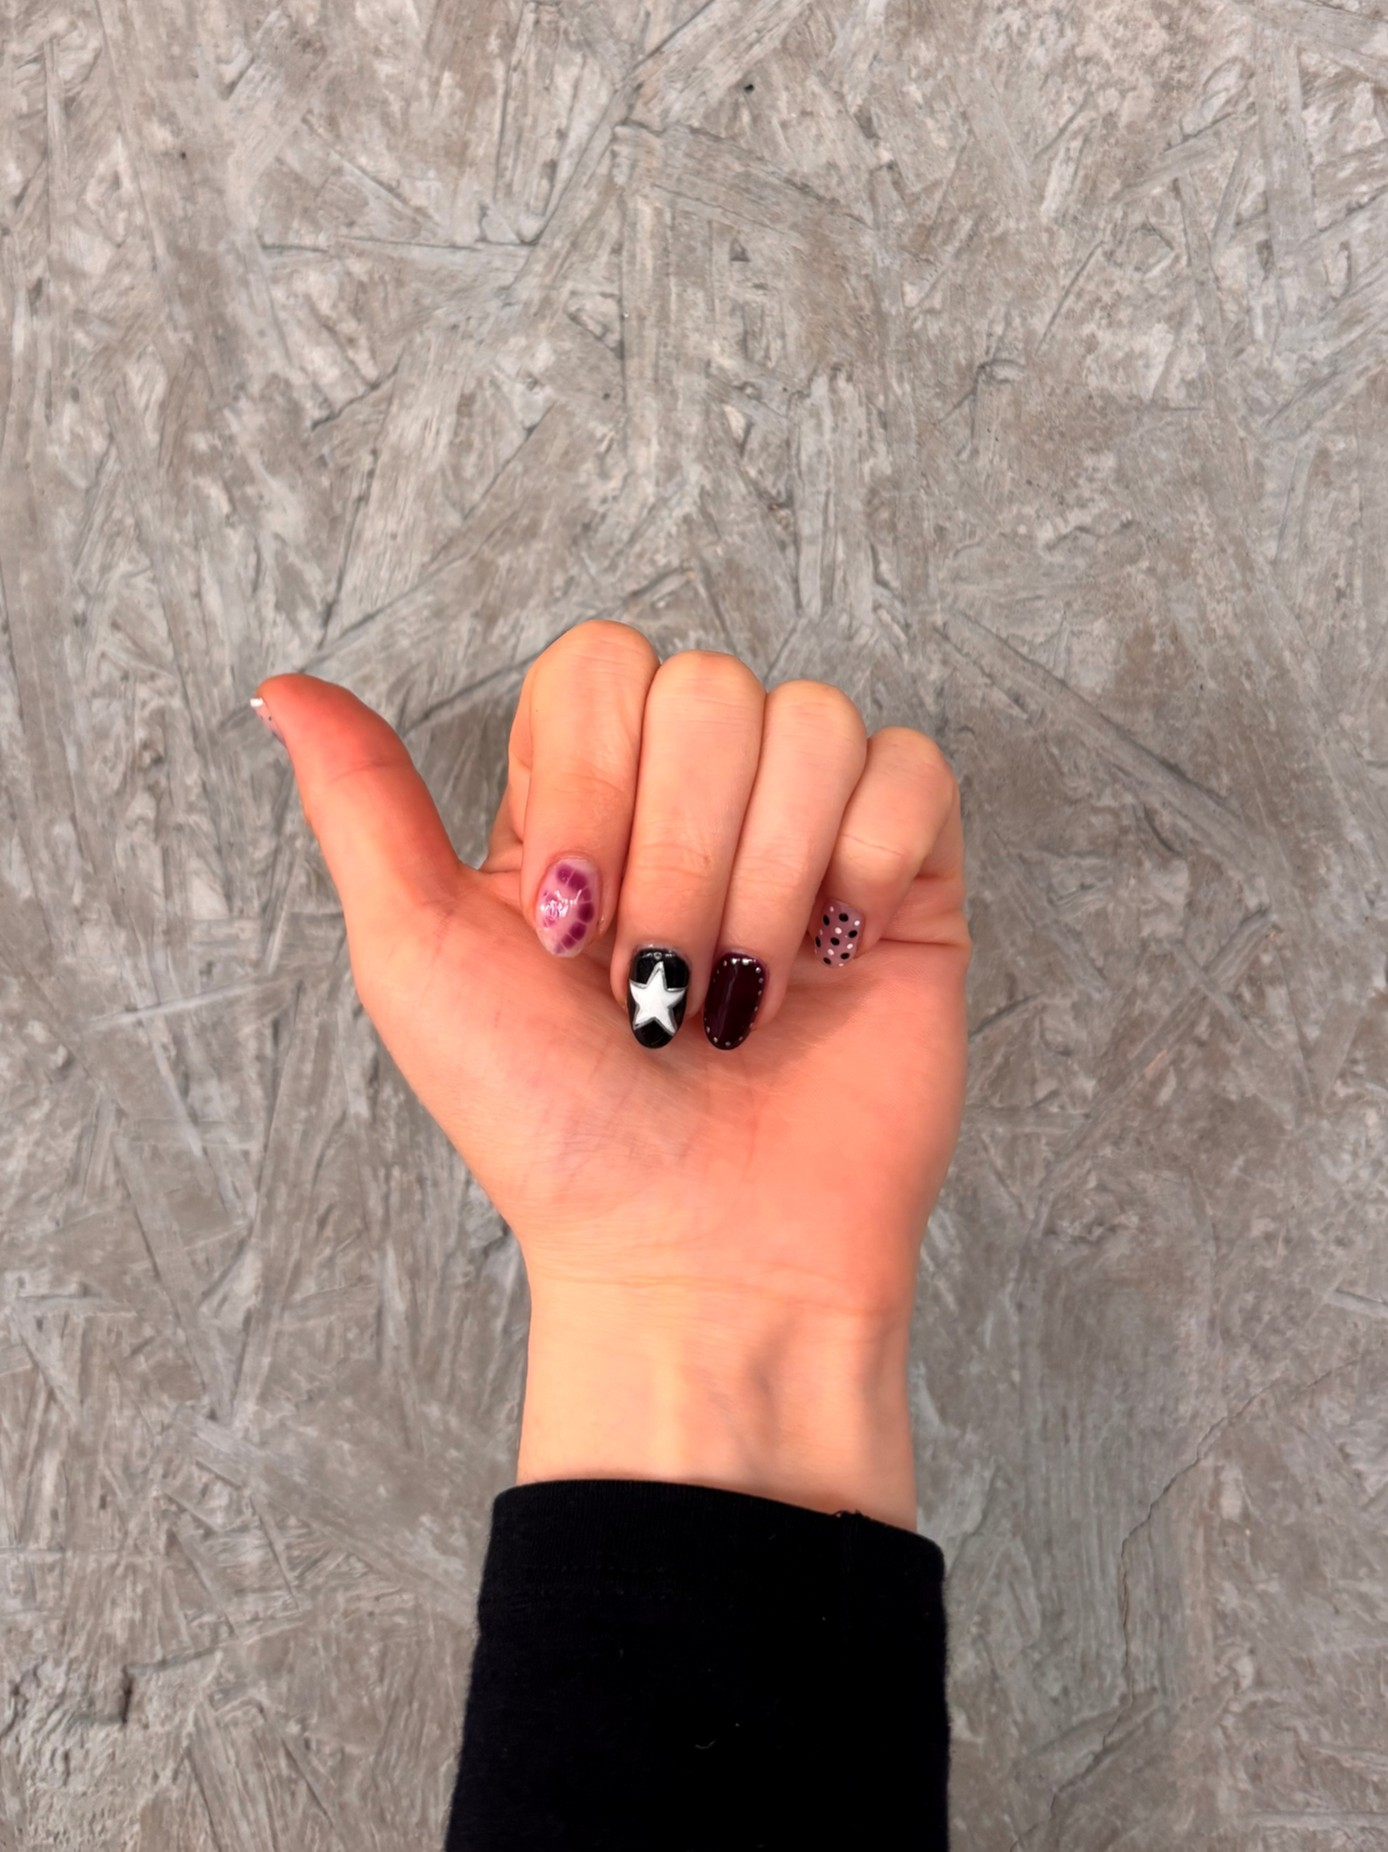
\includegraphics[
            width=\linewidth
        ]{content/images/grab_gesture.jpg}
        \caption{Grab-Geste}
        \label{fig:grab_gesture}
    \end{subfigure}
    \hspace{0.5cm}
    \begin{subfigure}[t]{0.6\textwidth}
        \centering
        
\includegraphics[
            width=\linewidth
        ]{content/images/grab_hint.png}
        \caption{Hinweisanimation, die Nutzer:innen zeigt, wie Dwell-Zeit übersprungen werden kann.}
        \label{fig:grab_hint}
    \end{subfigure}
    \caption{Darstellung der Grab-Interaktion.}
    \label{fig:grab}
\end{figure}

Durch die Kombination beider Mechanismen kann das System sowohl Einsteiger als auch erfahrene Nutzer:innen unterstützen.


\subsubsection{Visuelle Gestaltung und Zustandsrückmeldungen}

Da Mid-Air-Interaktion im Unterschied zu physischen Eingabegeräten keine direkte haptische Rückmeldung bietet, kommt der visuellen Kommunikation von Interaktionszuständen eine zentrale Rolle zu. Das Interaktionssystem sieht daher vor, relevante Zustände wie Fokussierung, Auswahl und laufende Aktivierung sichtbar zu machen. Dadurch soll jederzeit nachvollziehbar bleiben, welche Funktion aktuell adressiert wird und in welchem Zustand sich die Interaktion befindet.

Diese Form der Rückmeldung ist insbesondere vor dem Hintergrund der in Abschnitt~\ref{sec:rw_midair} beschriebenen Herausforderungen hinsichtlich Präzision, Kontrolle und Fehlinterpretation relevant. Visuelle Hinweise dienen hier nicht nur der Bestätigung erfolgreicher Eingaben, sondern auch der Reduktion von Unsicherheit während der Interaktion.

Es es sinnvoll mehrere visuelle Zustände zu planen, um den aktuellen Interaktionsstatus nachvollziehbar darzustellen. Befindet sich der Cursor über einem Menüsegment, wird dieses visuell hervorgehoben (Hover-Zustand, vgl. Abb. \ref{fig:zustandsvisualisierungen_synthese}, c). Diese Hervorhebung dient als unmittelbare Rückmeldung darüber, welches Menüelement aktuell fokussiert ist.

Wird ein Menüeintrag aktiv ausgewählt, durch eine Greifgeste oder durch das Auslösen eines Dwell-Timers, wechselt das entsprechende Segment in einen ausgewählten Zustand (Abb. \ref{fig:zustandsvisualisierungen_synthese}, b), der durch eine deutlichere Farbänderung dargestellt wird.

Während der Dwell-basierten Auswahl wird zusätzlich eine visuelle Fortschrittsanzeige eingeblendet.
Diese zeigt den zeitlichen Fortschritt der Aktivierung und ermöglicht es Nutzer:innen, den aktuellen Interaktionsstatus besser einzuschätzen (Abb. \ref{fig:zustandsvisualisierungen_synthese}, d).

{\color{red} TODO: ggf hier alte Visualisierung nehmen, wo ich noch Rahmen + pink hatte, damit implizit klar wird, dass es iterativer Stylingprozess war?}
\begin{figure}[H]
    \centering
    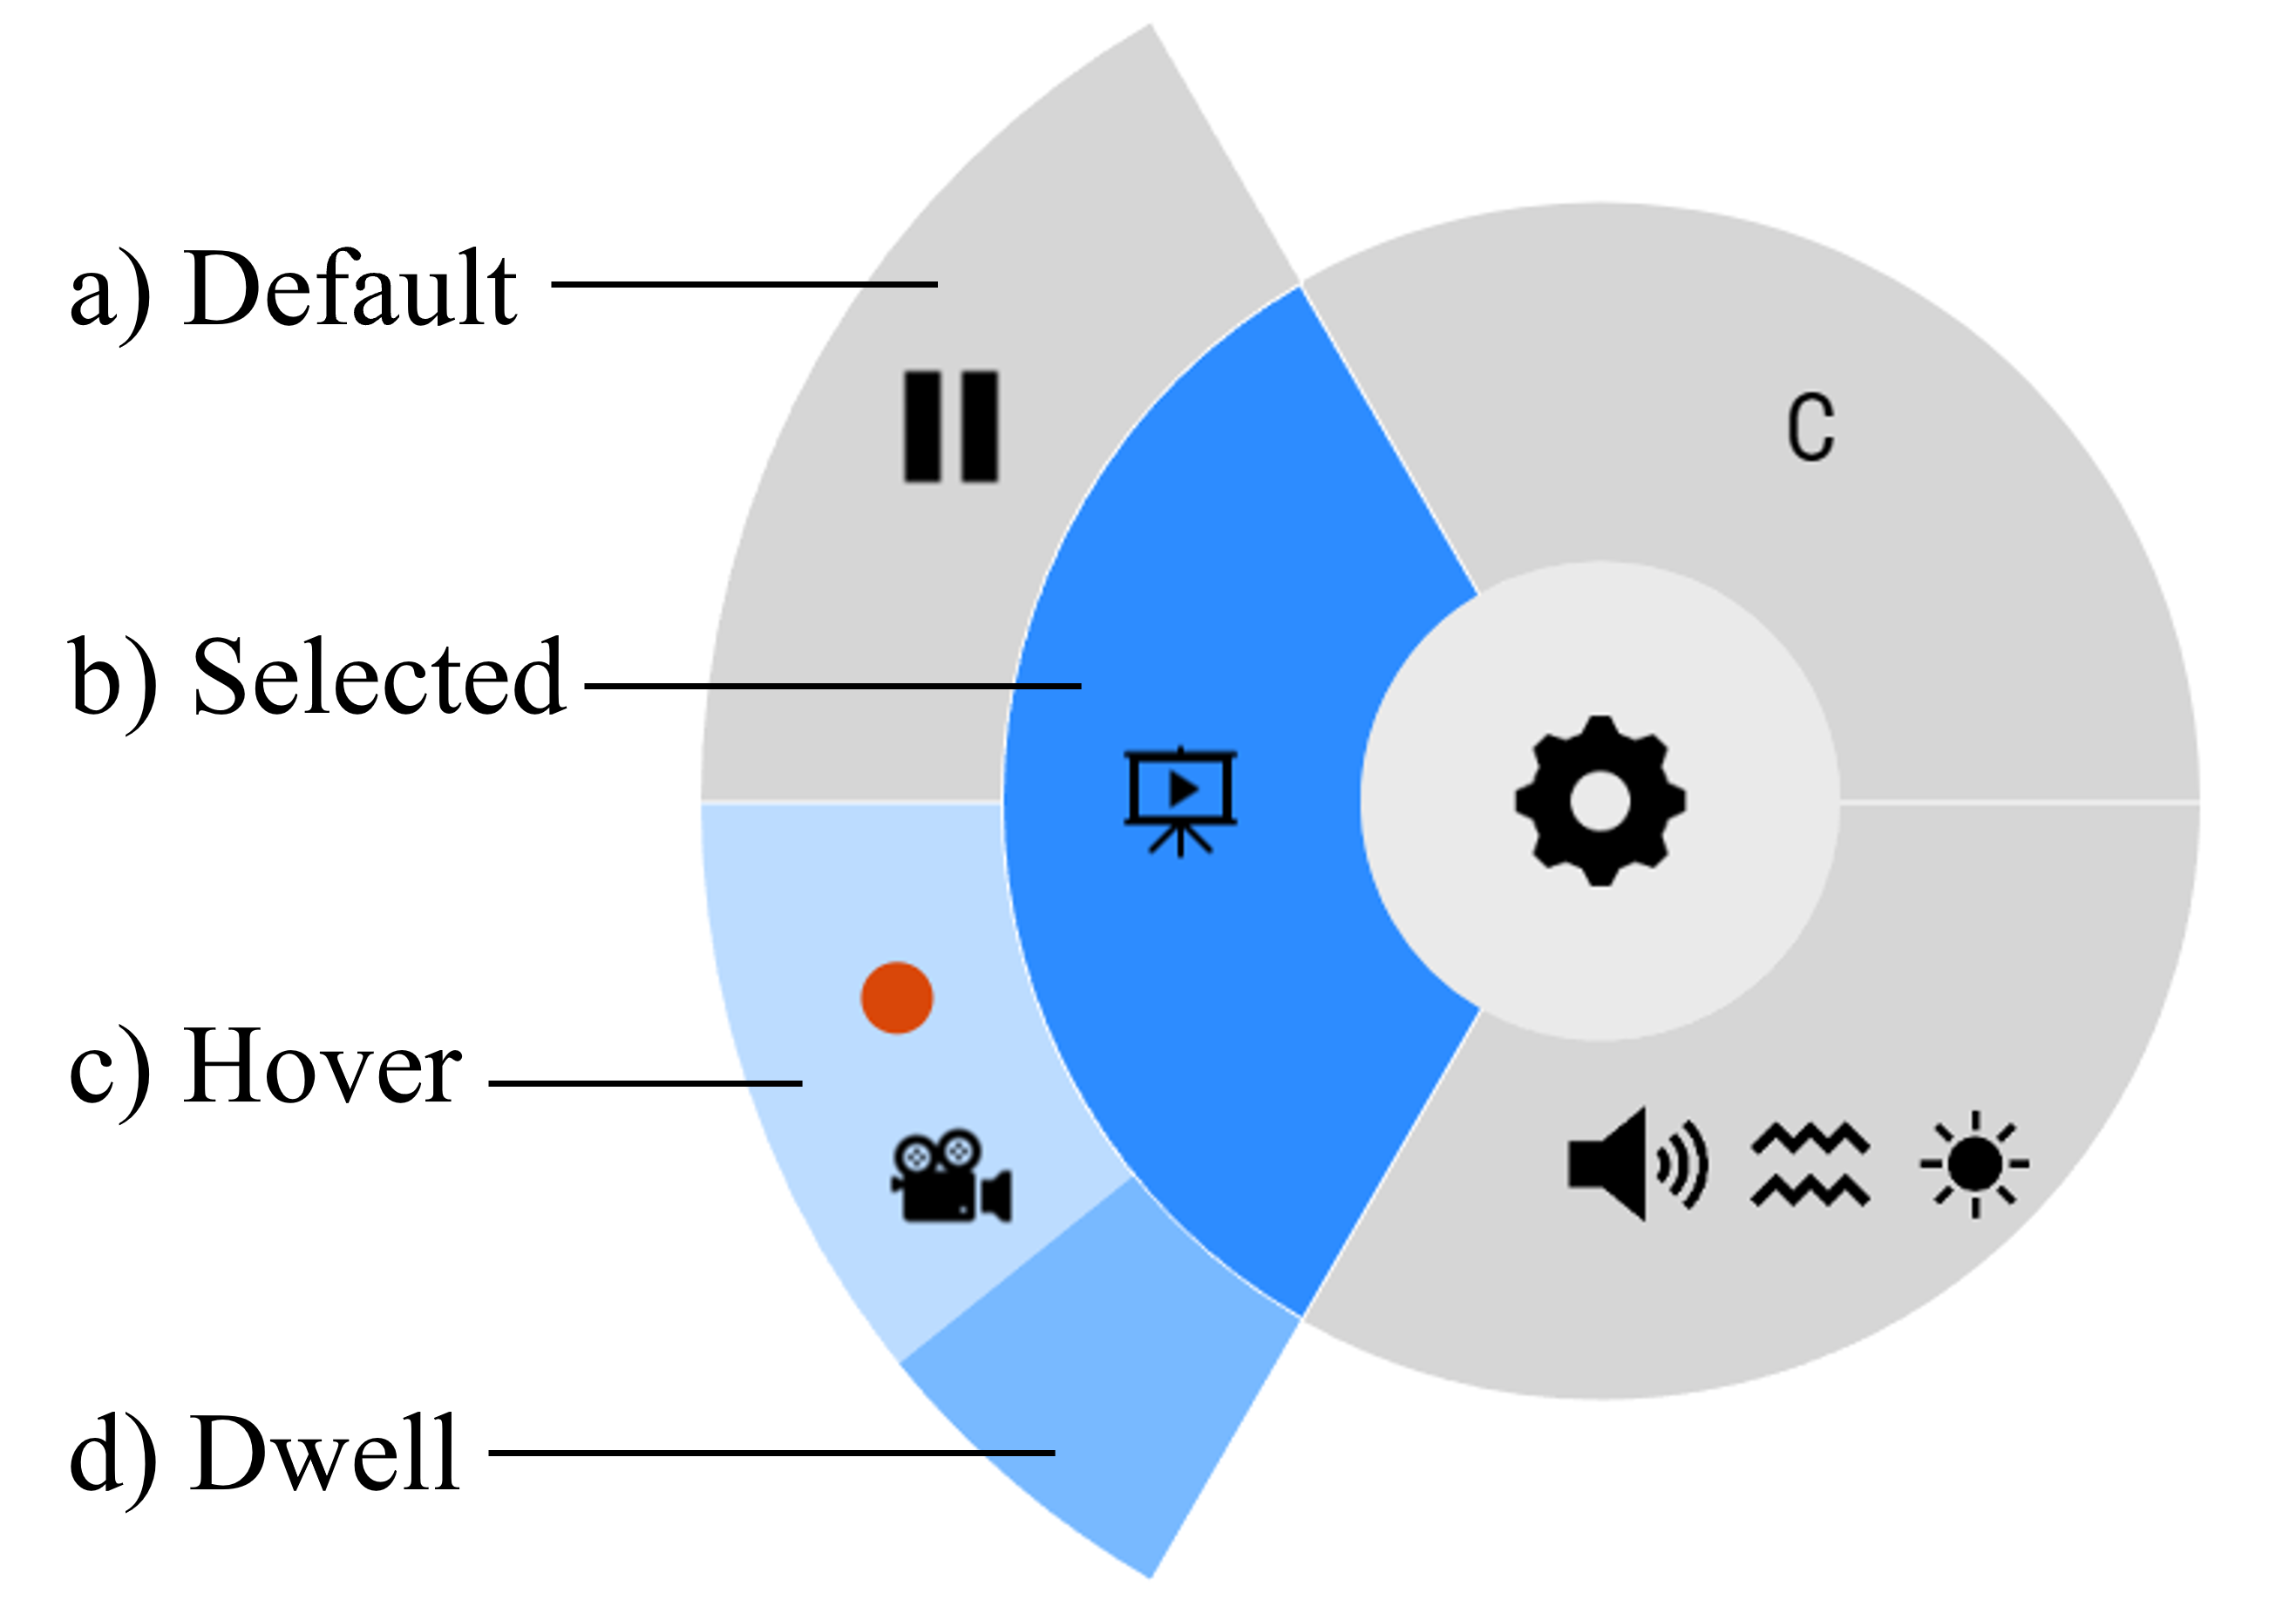
\includegraphics[width=0.5\linewidth]{content/diagrams/zustandsvisualisierungen.png}
    \caption{Verschiedene Visualisierungen des Zustands}
    \label{fig:zustandsvisualisierungen_synthese}
\end{figure}

Die konkrete visuelle Ausgestaltung wurde im Entwicklungsverlauf iterativ verfeinert.


\subsubsection{Submenus}
Um eine größere Anzahl von Funktionen innerhalb des Interaktionssystems zugänglich zu machen, wurde das radiale Menü um Submenüs erweitert. Einzelne Segmente des Hauptmenüs können weitere Menüebenen enthalten, die bei Auswahl eines Elements geöffnet werden.
Diese hierarchische Struktur ermöglicht es, thematisch zusammengehörige Funktionen zu gruppieren und gleichzeitig die visuelle Komplexität des Hauptmenüs zu reduzieren.
Menüeinträge erfüllen dabei zwei unterschiedliche Rollen: Sie können entweder als Kategorie fungieren (Abb. \ref{fig:menu_with_submenu_syn}) und ein weiteres Untermenü öffnen oder direkt eine Interaktion auslösen. Solche Interaktionen können beispielsweise diskrete Aktionen (zum Beispiel Button-Funktionen, vgl. Abb. \ref{fig:menu_with_button_syn}) oder kontinuierliche Parametersteuerungen wie Slider umfassen (Abb. \ref{fig:menu_with_slider_presentation_syn}).
Durch diese mehrstufige Organisation bleibt die Anzahl der gleichzeitig sichtbaren Menüelemente begrenzt, wodurch die Orientierung im Menü erleichtert wird und die Interaktion auch im Mid-Air-Kontext übersichtlich bleibt. Gleichzeitig erlaubt die hierarchische Struktur eine flexible Erweiterung des Systems um zusätzliche Funktionen.

\begin{figure}[H]
    \centering
    \begin{subfigure}[t]{0.3\textwidth}
        \centering
        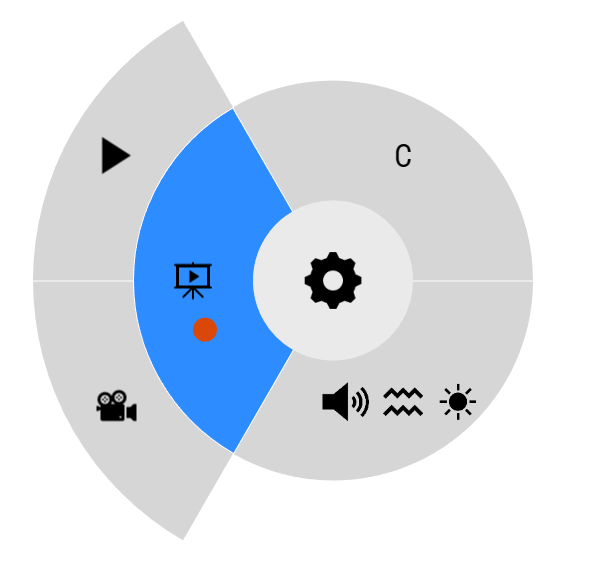
\includegraphics[width=\linewidth]{content/images/menu_with_submenu.png}
        \caption{Cursor befindet sich auf Menüelement, das ein Submenü öffnet.}
        \label{fig:menu_with_submenu_syn}
    \end{subfigure}
    \hfill
    \begin{subfigure}[t]{0.35\textwidth}
        \centering
        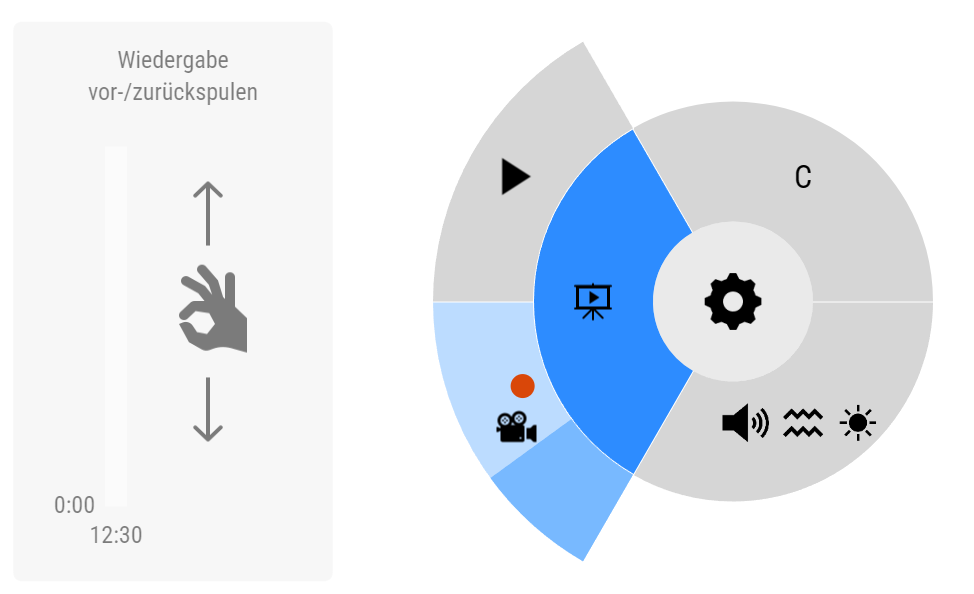
\includegraphics[width=\linewidth]{content/images/menu_with_slider_presentation.png}
        \caption{Cursor befindet sich auf Menüelement, das Slider öffnet.}
        \label{fig:menu_with_slider_presentation_syn}
    \end{subfigure}
    \hfill
    \begin{subfigure}[t]{0.3\textwidth}
        \centering
        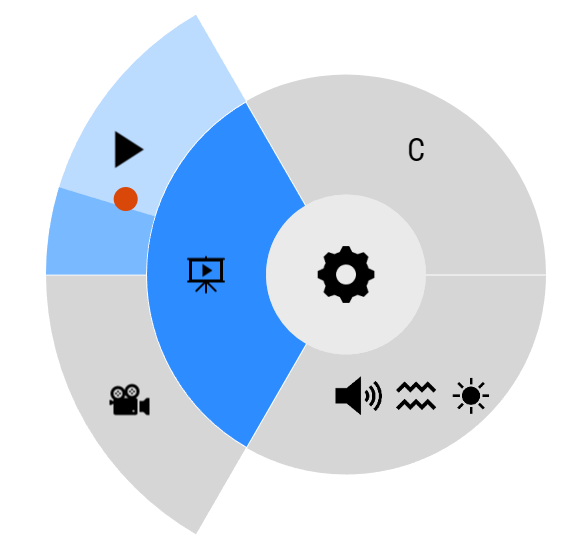
\includegraphics[width=\linewidth]{content/images/menu_with_button.png}
        \caption{Cursor befindet sich auf Menüelement, das als Button fungiert}
        \label{fig:menu_with_button_syn}
    \end{subfigure}
    \caption{Verschiedene Möglichkeit der Menüelemente}
    \label{fig:gesture_images_syn}
\end{figure}

Zum Aktivieren eines Untermenüs selektieren die Nutzer:innen einen Menüeintrag, der in der Menüstruktur über Kindelemente verfügt. Solange sich der Cursor innerhalb dieses Eintrags (Abb. \ref{fig:menu_cursor1}) oder des geöffneten Untermenüs (Abb. \ref{fig:menu_cursor2}) befindet, bleibt das Untermenü sichtbar und kann weiter genutzt werden.
Verlässt der Cursor sowohl den Menüeintrag als auch das zugehörige Untermenü (Abb. \ref{fig:menu_cursor3}), wird das Untermenü automatisch geschlossen. Durch diese kontextabhängige Sichtbarkeit bleibt die visuelle Komplexität des Menüs gering, während gleichzeitig eine größere Anzahl von Funktionen selektiv zugänglich gemacht werden kann.

\begin{figure}[H]
    \centering
    \begin{subfigure}[t]{0.32\textwidth}
        \centering
        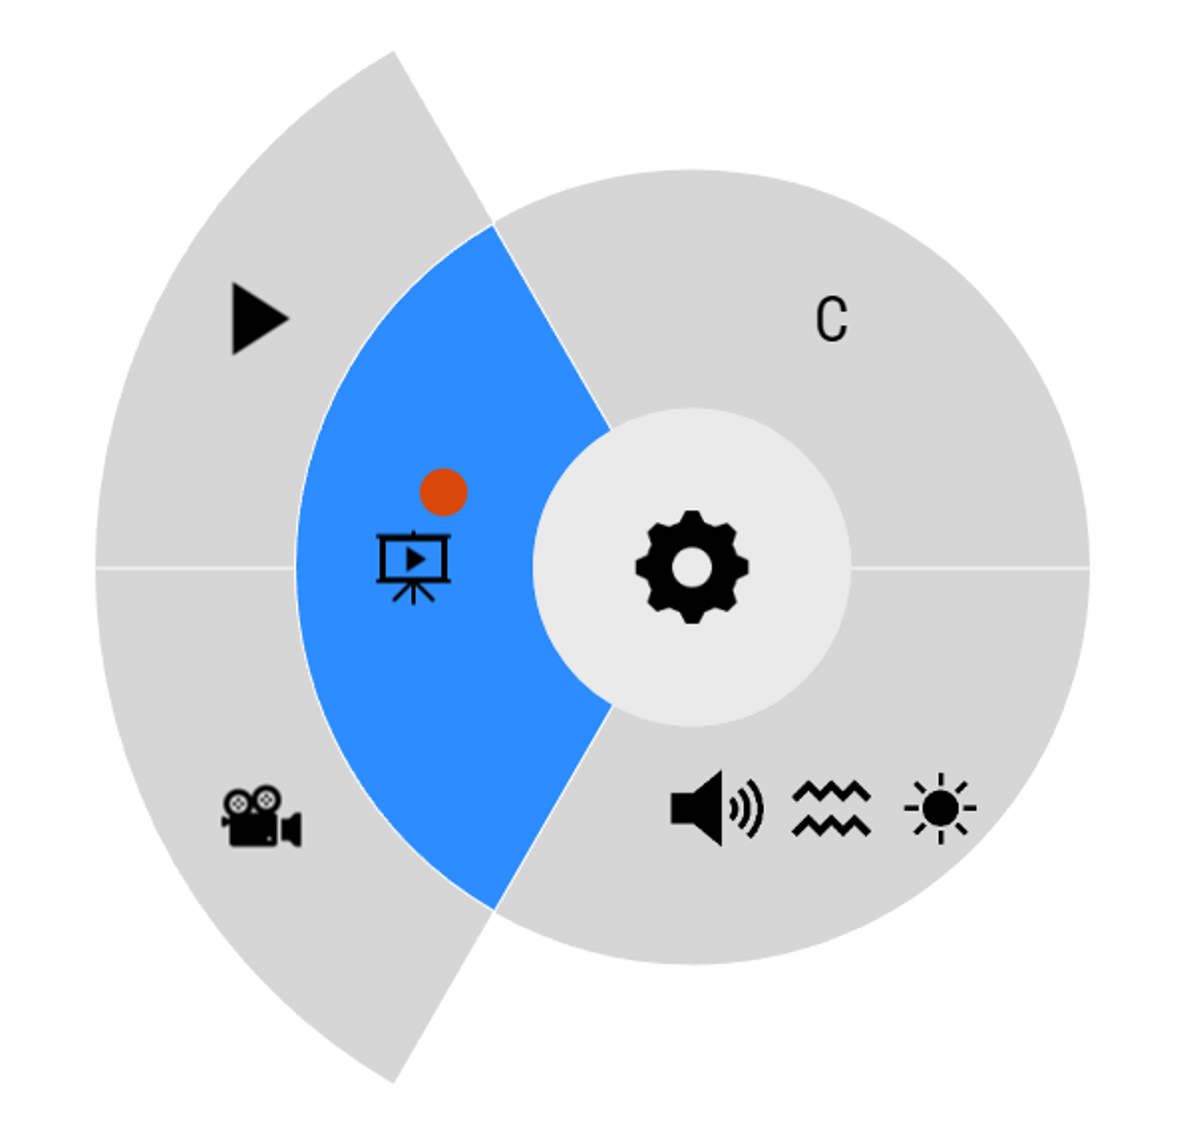
\includegraphics[width=\linewidth]{content/images/menu_cursor1.png}
        \caption{Cursor in Hauptmenüelement, nachdem Submenü geöffnet wurde.}
        \label{fig:menu_cursor1}
    \end{subfigure}
    \hfill
    \begin{subfigure}[t]{0.32\textwidth}
        \centering
        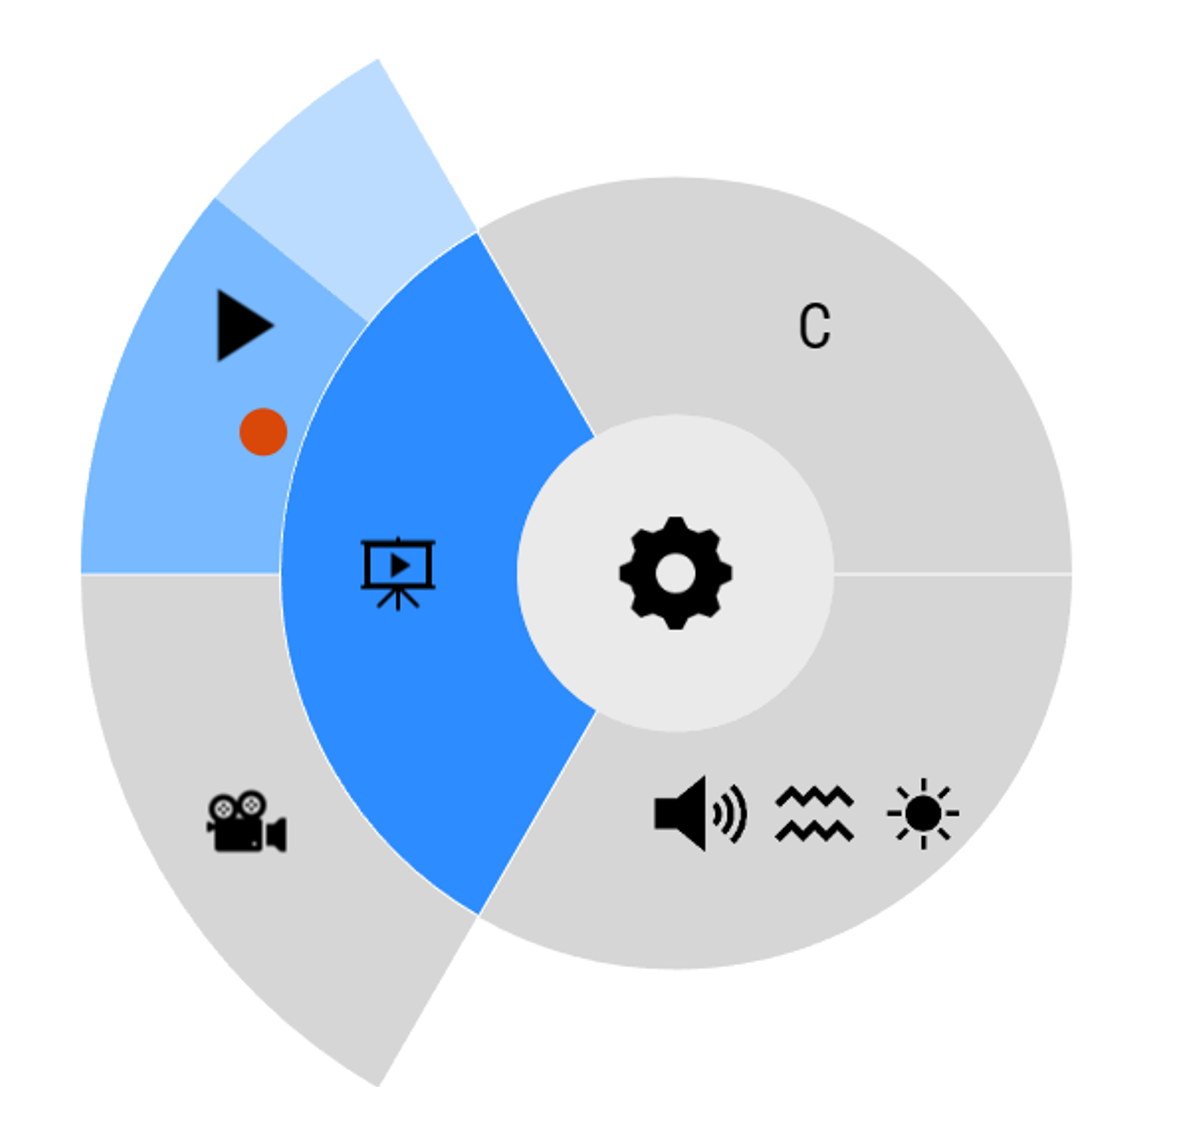
\includegraphics[width=\linewidth]{content/images/menu_cursor2.png}
        \caption{Cursor in Submenü.}
        \label{fig:menu_cursor2}
    \end{subfigure}
    \hfill
    \begin{subfigure}[t]{0.32\textwidth}
        \centering
        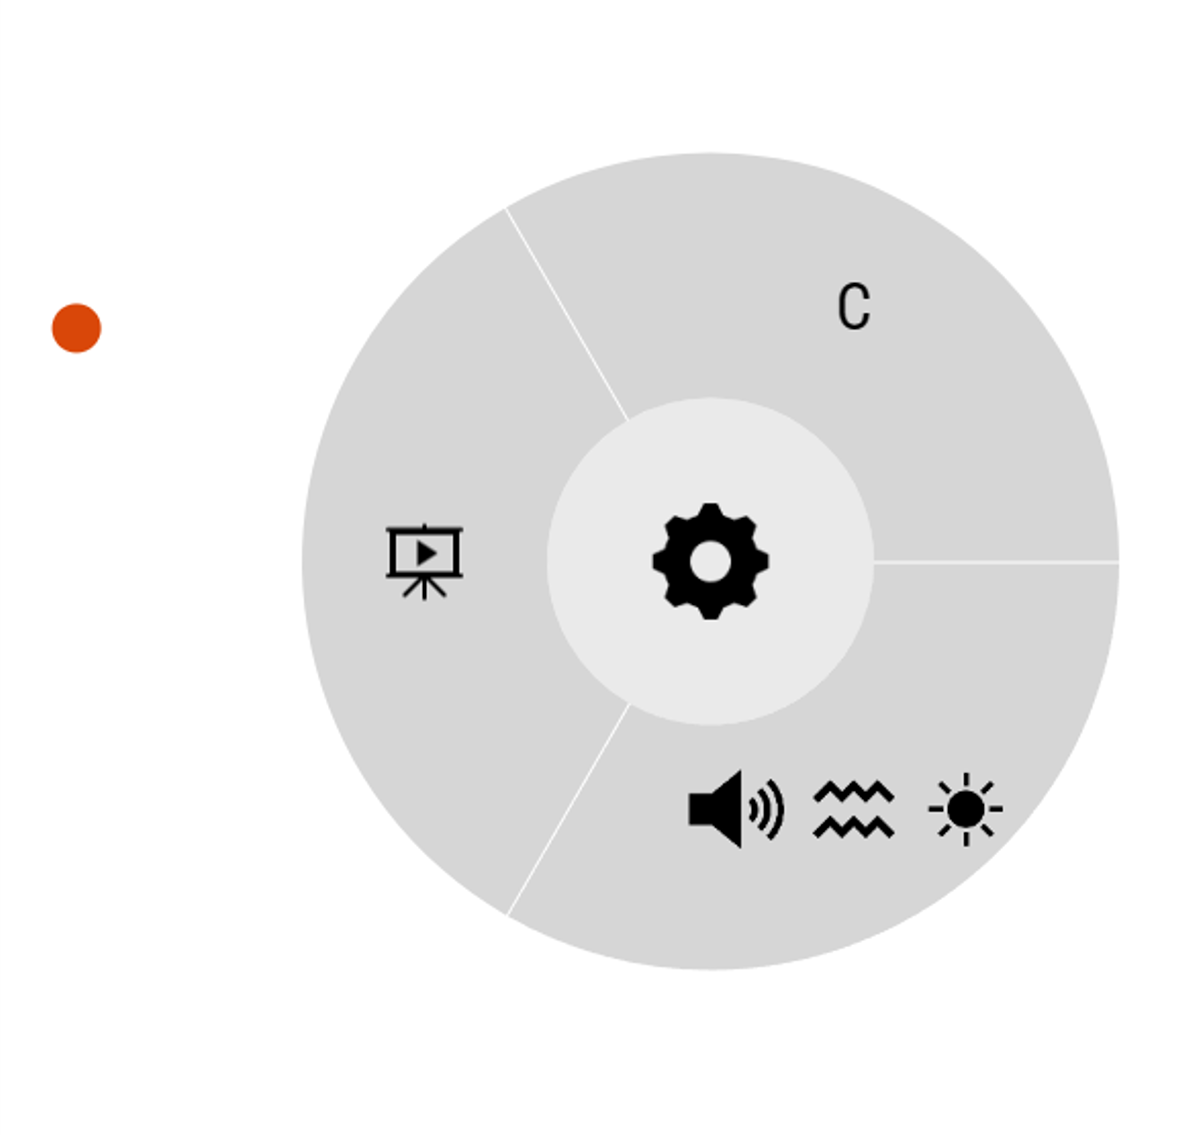
\includegraphics[width=\linewidth]{content/images/menu_cursor3.png}
        \caption{Cursor ist aus Submenü herausnavigiert, woraufhin sich Submenü geschlossen hat.}
        \label{fig:menu_cursor3}
    \end{subfigure}
    \caption{Zustandsdarstellungen der Submenü-Sichtbarkeitslogik {\color{red} Braucht man die Visualisierung oder checkt man das auch ohne?}}
    \label{fig:submenu}
\end{figure}

\subsubsection{Slider}
Während das radiale Menü insbesondere für diskrete Auswahlentscheidungen geeignet ist, erfordern kontinuierliche Parameter wie Lautstärke, Helligkeit oder Vibrationsintensität eine andere Form der Interaktion. Deshalb wurde das menübasierte Konzept um Slider als Mechanismus zur kontinuierlichen Steuerung erweitert.
Diese Erweiterung greift die in Abschnitt~\ref{sec:rw_menus} diskutierte Frage auf, wie Marking-Menu-artige Systeme über reine Befehlsauswahl hinaus auch zur feineren Parametersteuerung genutzt werden können. Das Ziel besteht darin, diskrete und kontinuierliche Interaktion innerhalb eines gemeinsamen Systems zu vereinen, anstatt für unterschiedliche Aufgaben vollständig getrennte Interaktionsparadigmen einzuführen.
Im Kontext des Marking-Menus erfolgt dies durch die Auswahl eines Menüeintrags, der bereits während des Hover-Zustands durch eine visuelle Vorschau auf die veränderte Interaktionsart hinweist (Abb.~\ref{fig:slider_preview}). Die reduzierte visuelle Hervorhebung signalisiert dabei, dass zunächst eine explizite Auswahl des Menüsegments erforderlich ist, um die Sliderinteraktion zu aktivieren. Nach Bestätigung der Auswahl wechselt das System in einen Anpassungsmodus, in dem der Parameter direkt verändert werden kann (Abb.~\ref{fig:slider_active}). In diesem Modus wird das Menü visuell zurückgenommen und der Cursor ausgeblendet, um den Fokus auf die Sliderinteraktion zu lenken.

\begin{figure}[H]
    \centering
    \begin{subfigure}{0.49\textwidth}
        \centering
        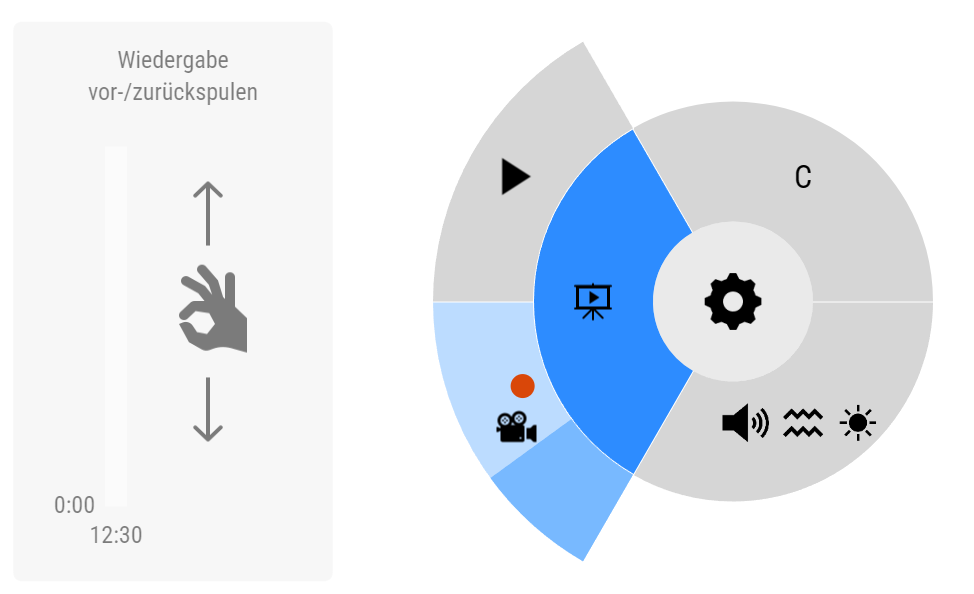
\includegraphics[width=\linewidth]{content/images/menu_with_slider_presentation.png}
        \caption{Vorschau}
        \label{fig:slider_preview}
    \end{subfigure}
    \hfill
    \begin{subfigure}{0.49\textwidth}
        \centering
        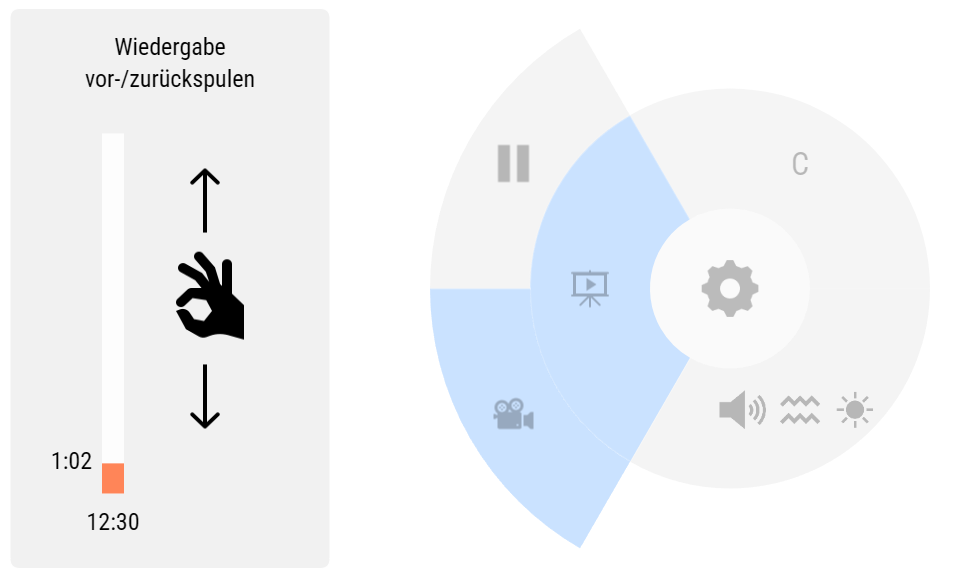
\includegraphics[width=\linewidth]{content/images/slider_active.png}
        \caption{Aktiver Zustand}
        \label{fig:slider_active}
    \end{subfigure}
    \caption{Darstellungen der verschiedenen Slider-Zustände}
    \label{fig:slider_states}
\end{figure}

Die Steuerung erfolgt über eine gezielte Handbewegung entlang einer definierten Interaktionsachse. Diese wird durch eine Pinch-Geste aktiviert, bei der Nutzer:innen den Parameter durch Verschieben der Hand entlang der jeweiligen Achse verändern. Die Kombination aus Aktivierungsgeste und anschließender gerichteter Bewegung greift Elemente von Micro-Gesten-basierten Interaktionen auf (vgl. Abschnitt~\ref{sec:rw_gestures} und Abschnitt~\ref{sec:rw_menus}). Um die Discoverability der Interaktion zu verbessern, wird im Sliderbereich eine visuelle Anleitung eingeblendet, die die Pinch-Geste sowie die mögliche Bewegungsrichtung verdeutlicht. Diese visuelle Unterstützung erleichtert insbesondere Erstnutzer:innen den Einstieg in die Interaktion.

Gleichzeitig greift die Interaktion eine vertraute physische Metapher auf: Das Verschieben des Sliders entspricht dem Greifen und Bewegen eines realen Reglers. Diese räumliche Analogie unterstützt eine intuitive Bedienung und ermöglicht es Nutzer:innen, die Interaktion durch Lösen der Pinch-Geste jederzeit zu beenden, wodurch eine kontrollierte und leicht verständliche Anpassung der Werte entsteht.

\begin{figure}[H]
    \centering
    \begin{subfigure}[t]{0.27\textwidth}
        \centering
        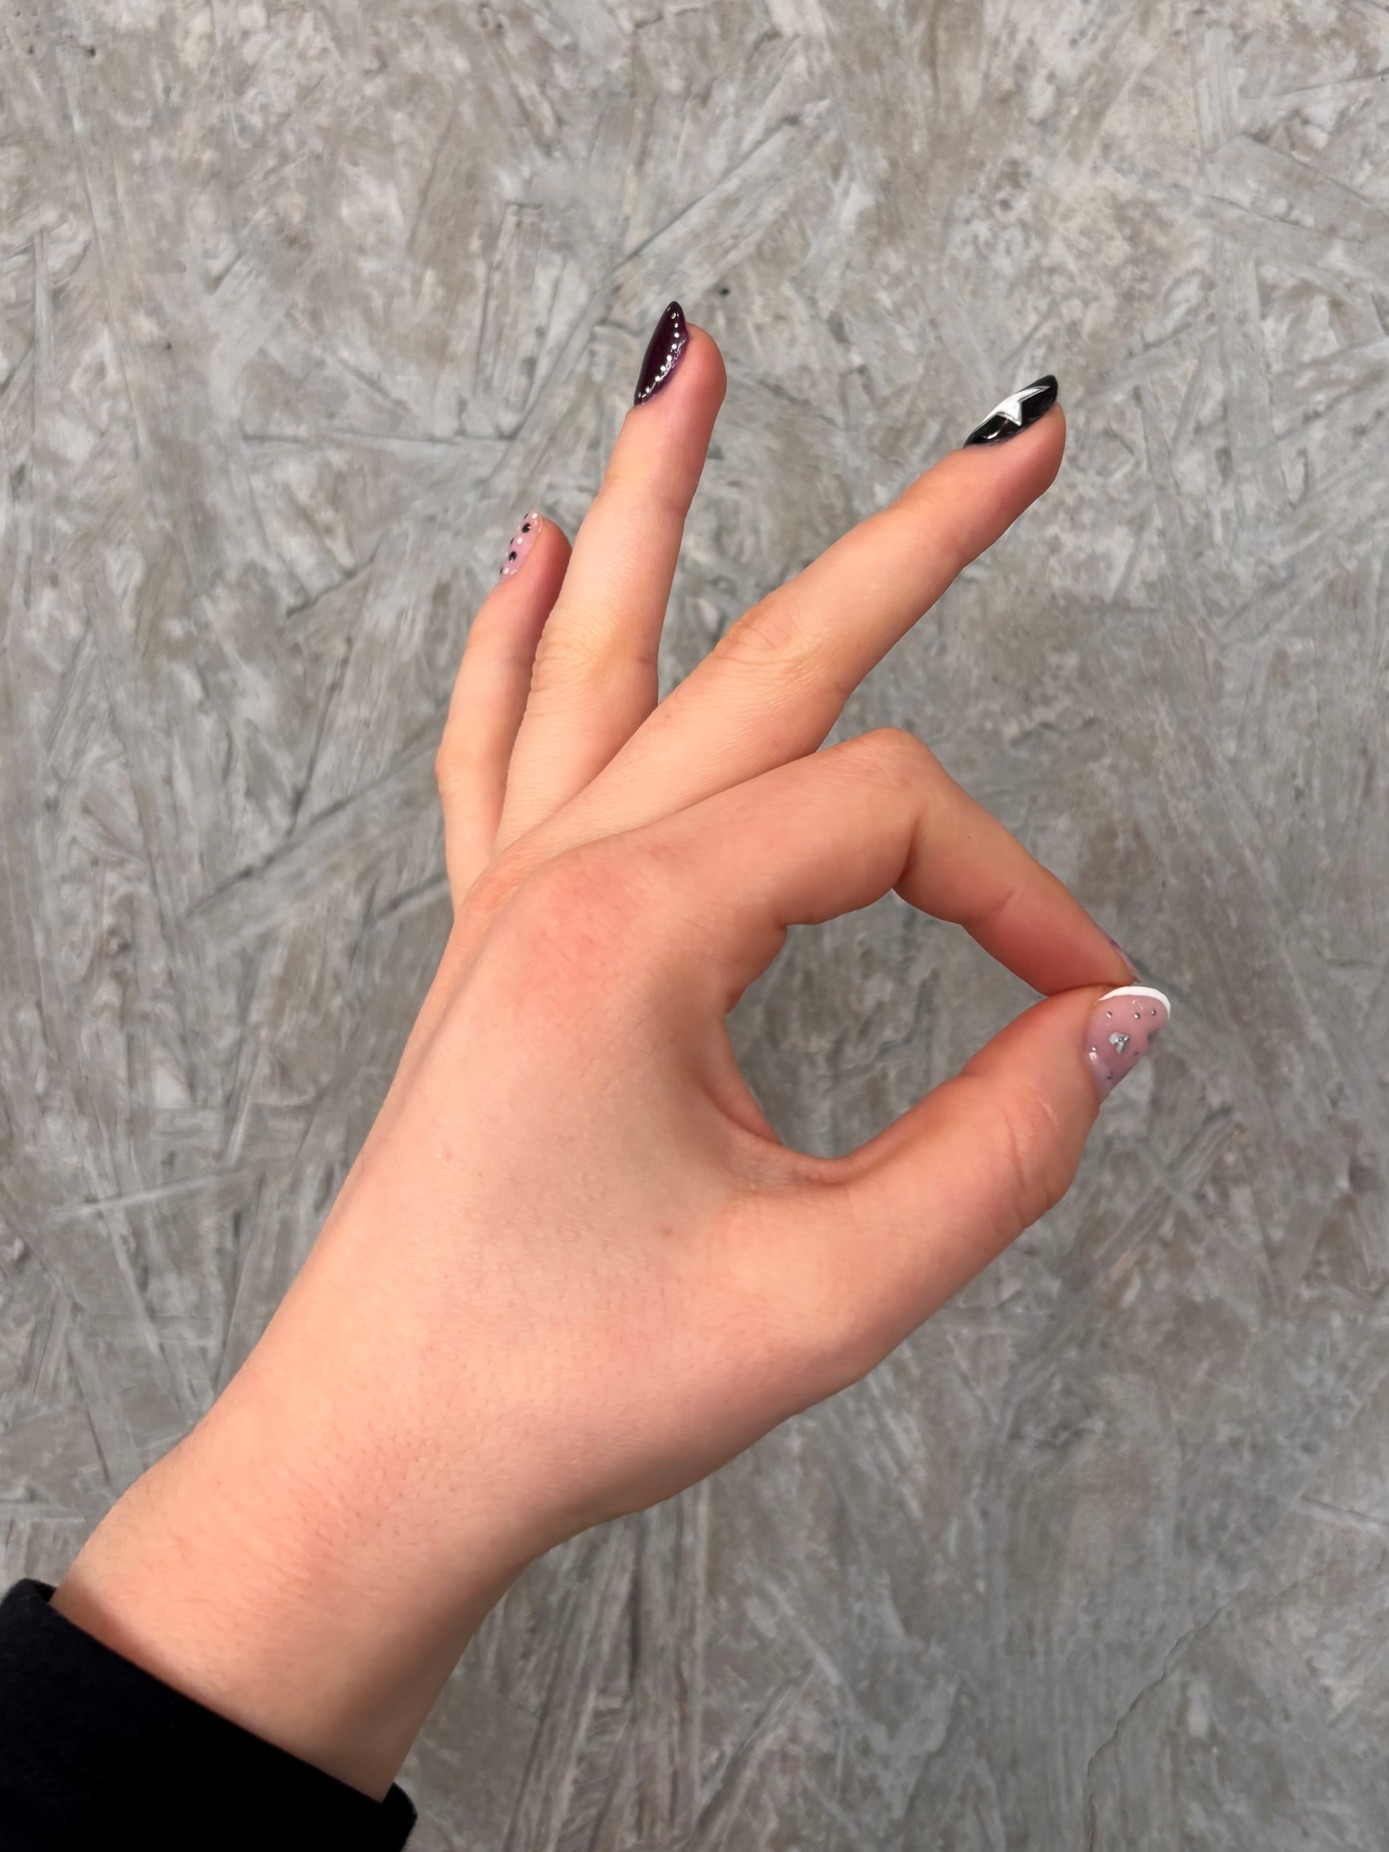
\includegraphics[width=\linewidth]{content/images/pinch_gesture.jpg}
        \caption{Pinch, bei dem aktiv ein Sliderwert verändert wird.}
        \label{fig:pinch_gesture}
    \end{subfigure}
    \hspace{0.5cm}
    \begin{subfigure}[t]{0.27\textwidth}
        \centering
        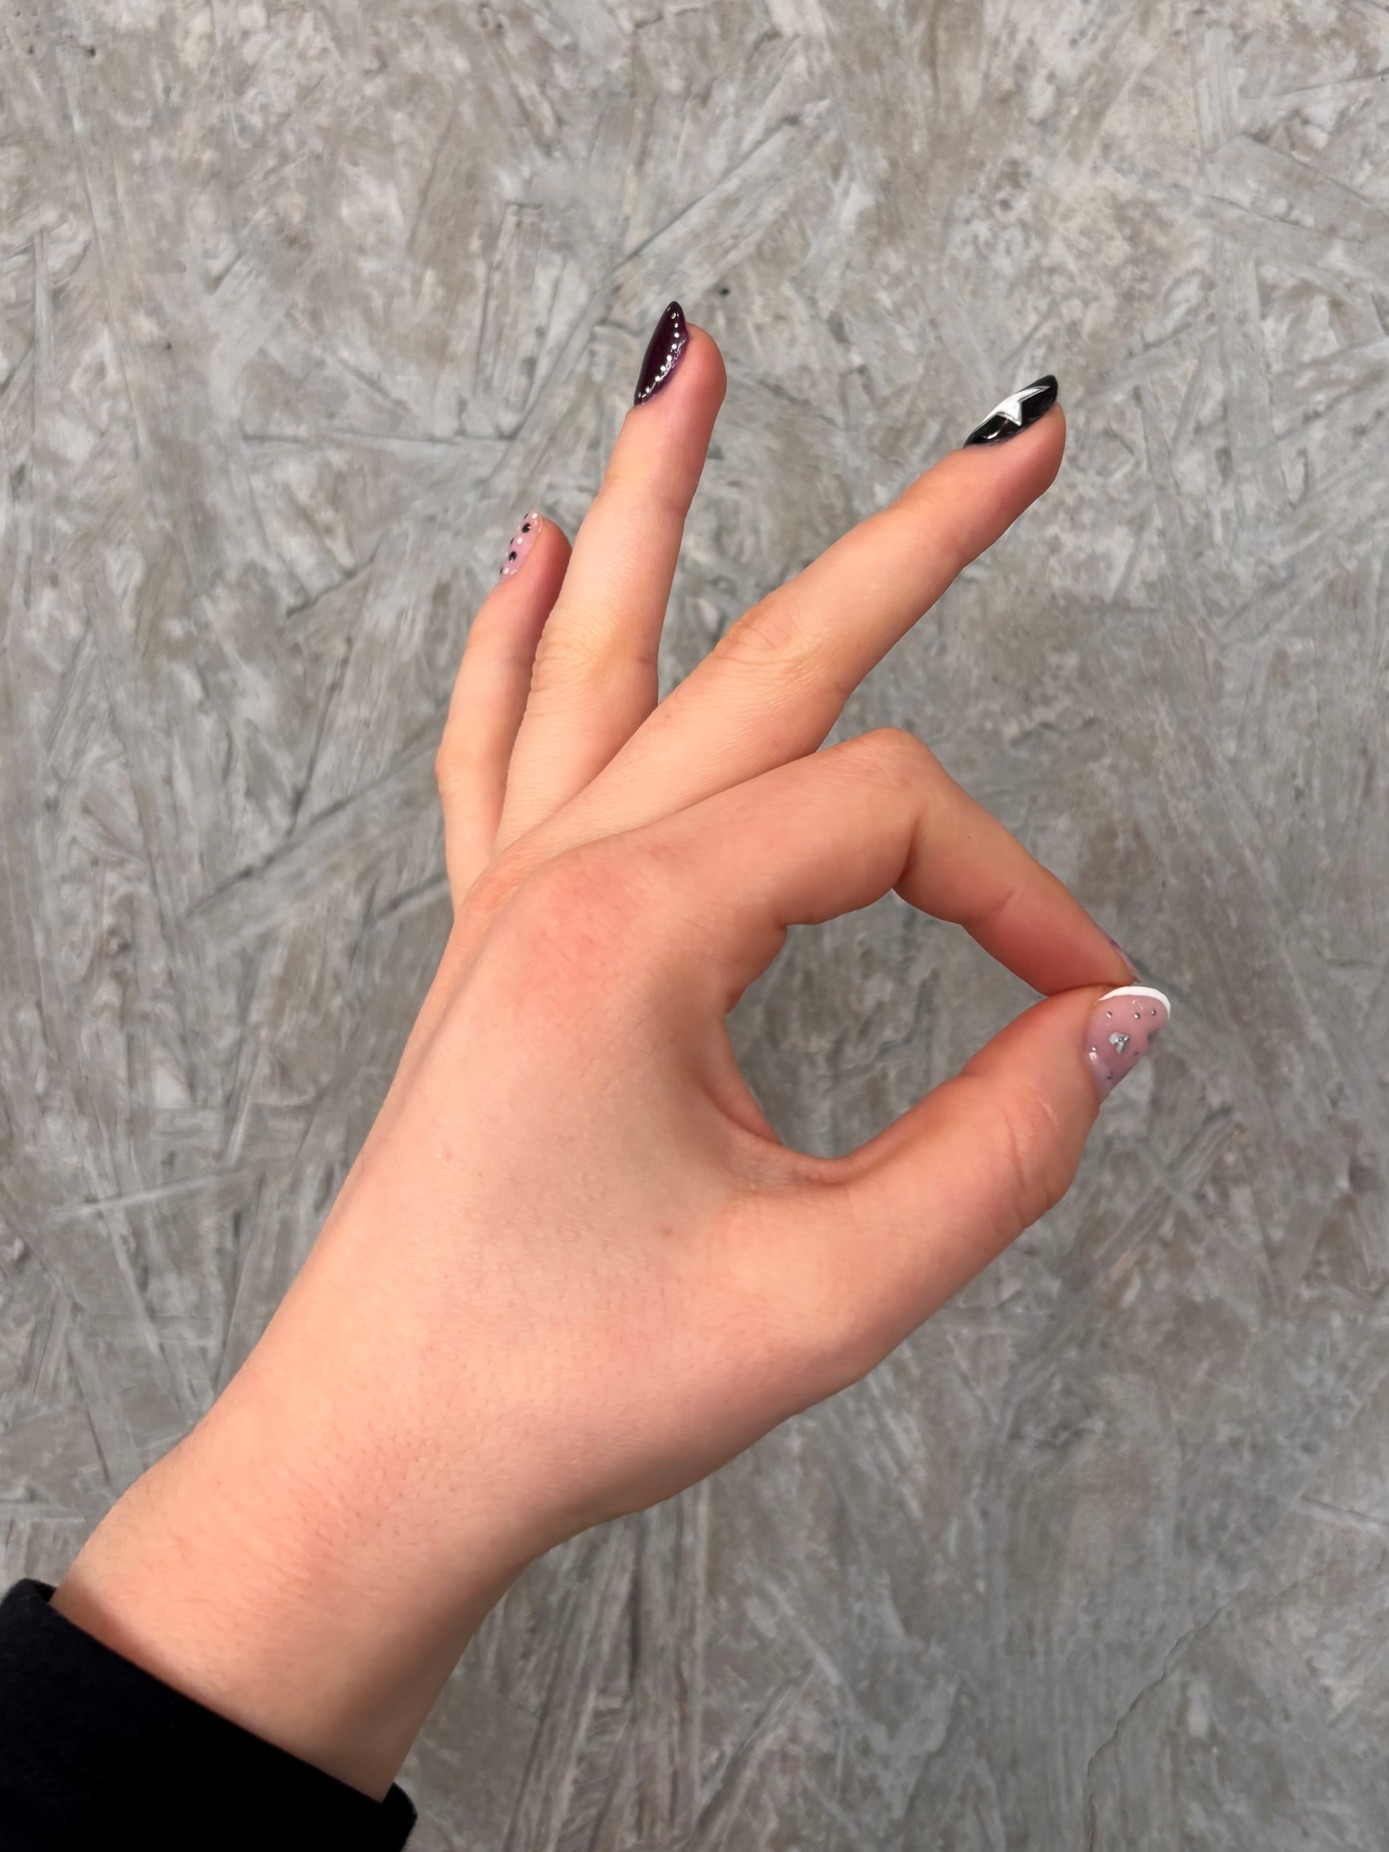
\includegraphics[width=\linewidth]{content/images/pinch_gesture.jpg}
        \caption{Geste, bei der der Sliderwert nicht aktiv verändert wird. {\color{red} TODO Foto von offenem Pinch machen!!}}
        \label{fig:pinch_gesture_open}
    \end{subfigure}
    \caption{Darstellungen der verschiedenen Pinch-Gestenzustände}
    \label{fig:pinch}
\end{figure}

Je nach Kontext und Menüeintrag wird die Position des Sliders relativ zum Menü angepasst. Der Slider kann dabei oberhalb, unterhalb oder seitlich des Menüs erscheinen, wodurch sich entweder eine horizontale oder vertikale Interaktionsachse ergibt. Entsprechend wird die Pinch-Geste entlang dieser Achse ausgeführt, sodass eine konsistente räumliche Zuordnung zwischen visueller Darstellung und Interaktionsbewegung entsteht.

Durch die Integration solcher Slider lassen sich kontinuierliche Parameter innerhalb des Interaktionssystems einheitlich steuern.


\subsubsection{Beispiele aktueller Interaktionen}
{\color{red} TODO: überlegen ob button doch in extra abschnitt muss, aber denke eigentlich nicht, weil es gibt ja nur den einen => dann eher generalisierbarkeit als todo in den ausblick }

Die Marking-Menu Interaktionen umfassen sowohl kontinuierliche Parametersteuerungen als auch diskrete Steuerungsfunktionen.
Ein zentraler Anwendungsfall für kontinuierliche Interaktion sind Slider zur Anpassung von Parametern wie Helligkeit, Vibration und Lautstärke. Diese werden in Form prozentualer Werte dargestellt und ermöglichen eine direkte, kontinuierliche Kontrolle der jeweiligen Systemparameter.

Darüber hinaus wird das Interaktionssystem zur Steuerung vorgerenderter Medieninhalte eingesetzt. In diesem Kontext dient ein Slider zur Navigation innerhalb eines Videos, indem er die aktuelle Abspielposition repräsentiert und gleichzeitig die Gesamtlänge des Materials visualisiert. Während der Wiedergabe bewegt sich der Slider automatisch entlang der Zeitleiste, wodurch der aktuelle Fortschritt kontinuierlich angezeigt wird.

Abbildung~\ref{fig:Slidertypen} zeigt beide Varianten im Vergleich. Während parameterbasierte Slider den aktuellen Wert als prozentuale Angabe darstellen, repräsentieren medienbezogene Slider eine zeitliche Position innerhalb eines Videos. Die zugrunde liegende Interaktionslogik bleibt dabei identisch.

\begin{figure}[H]
    \centering
    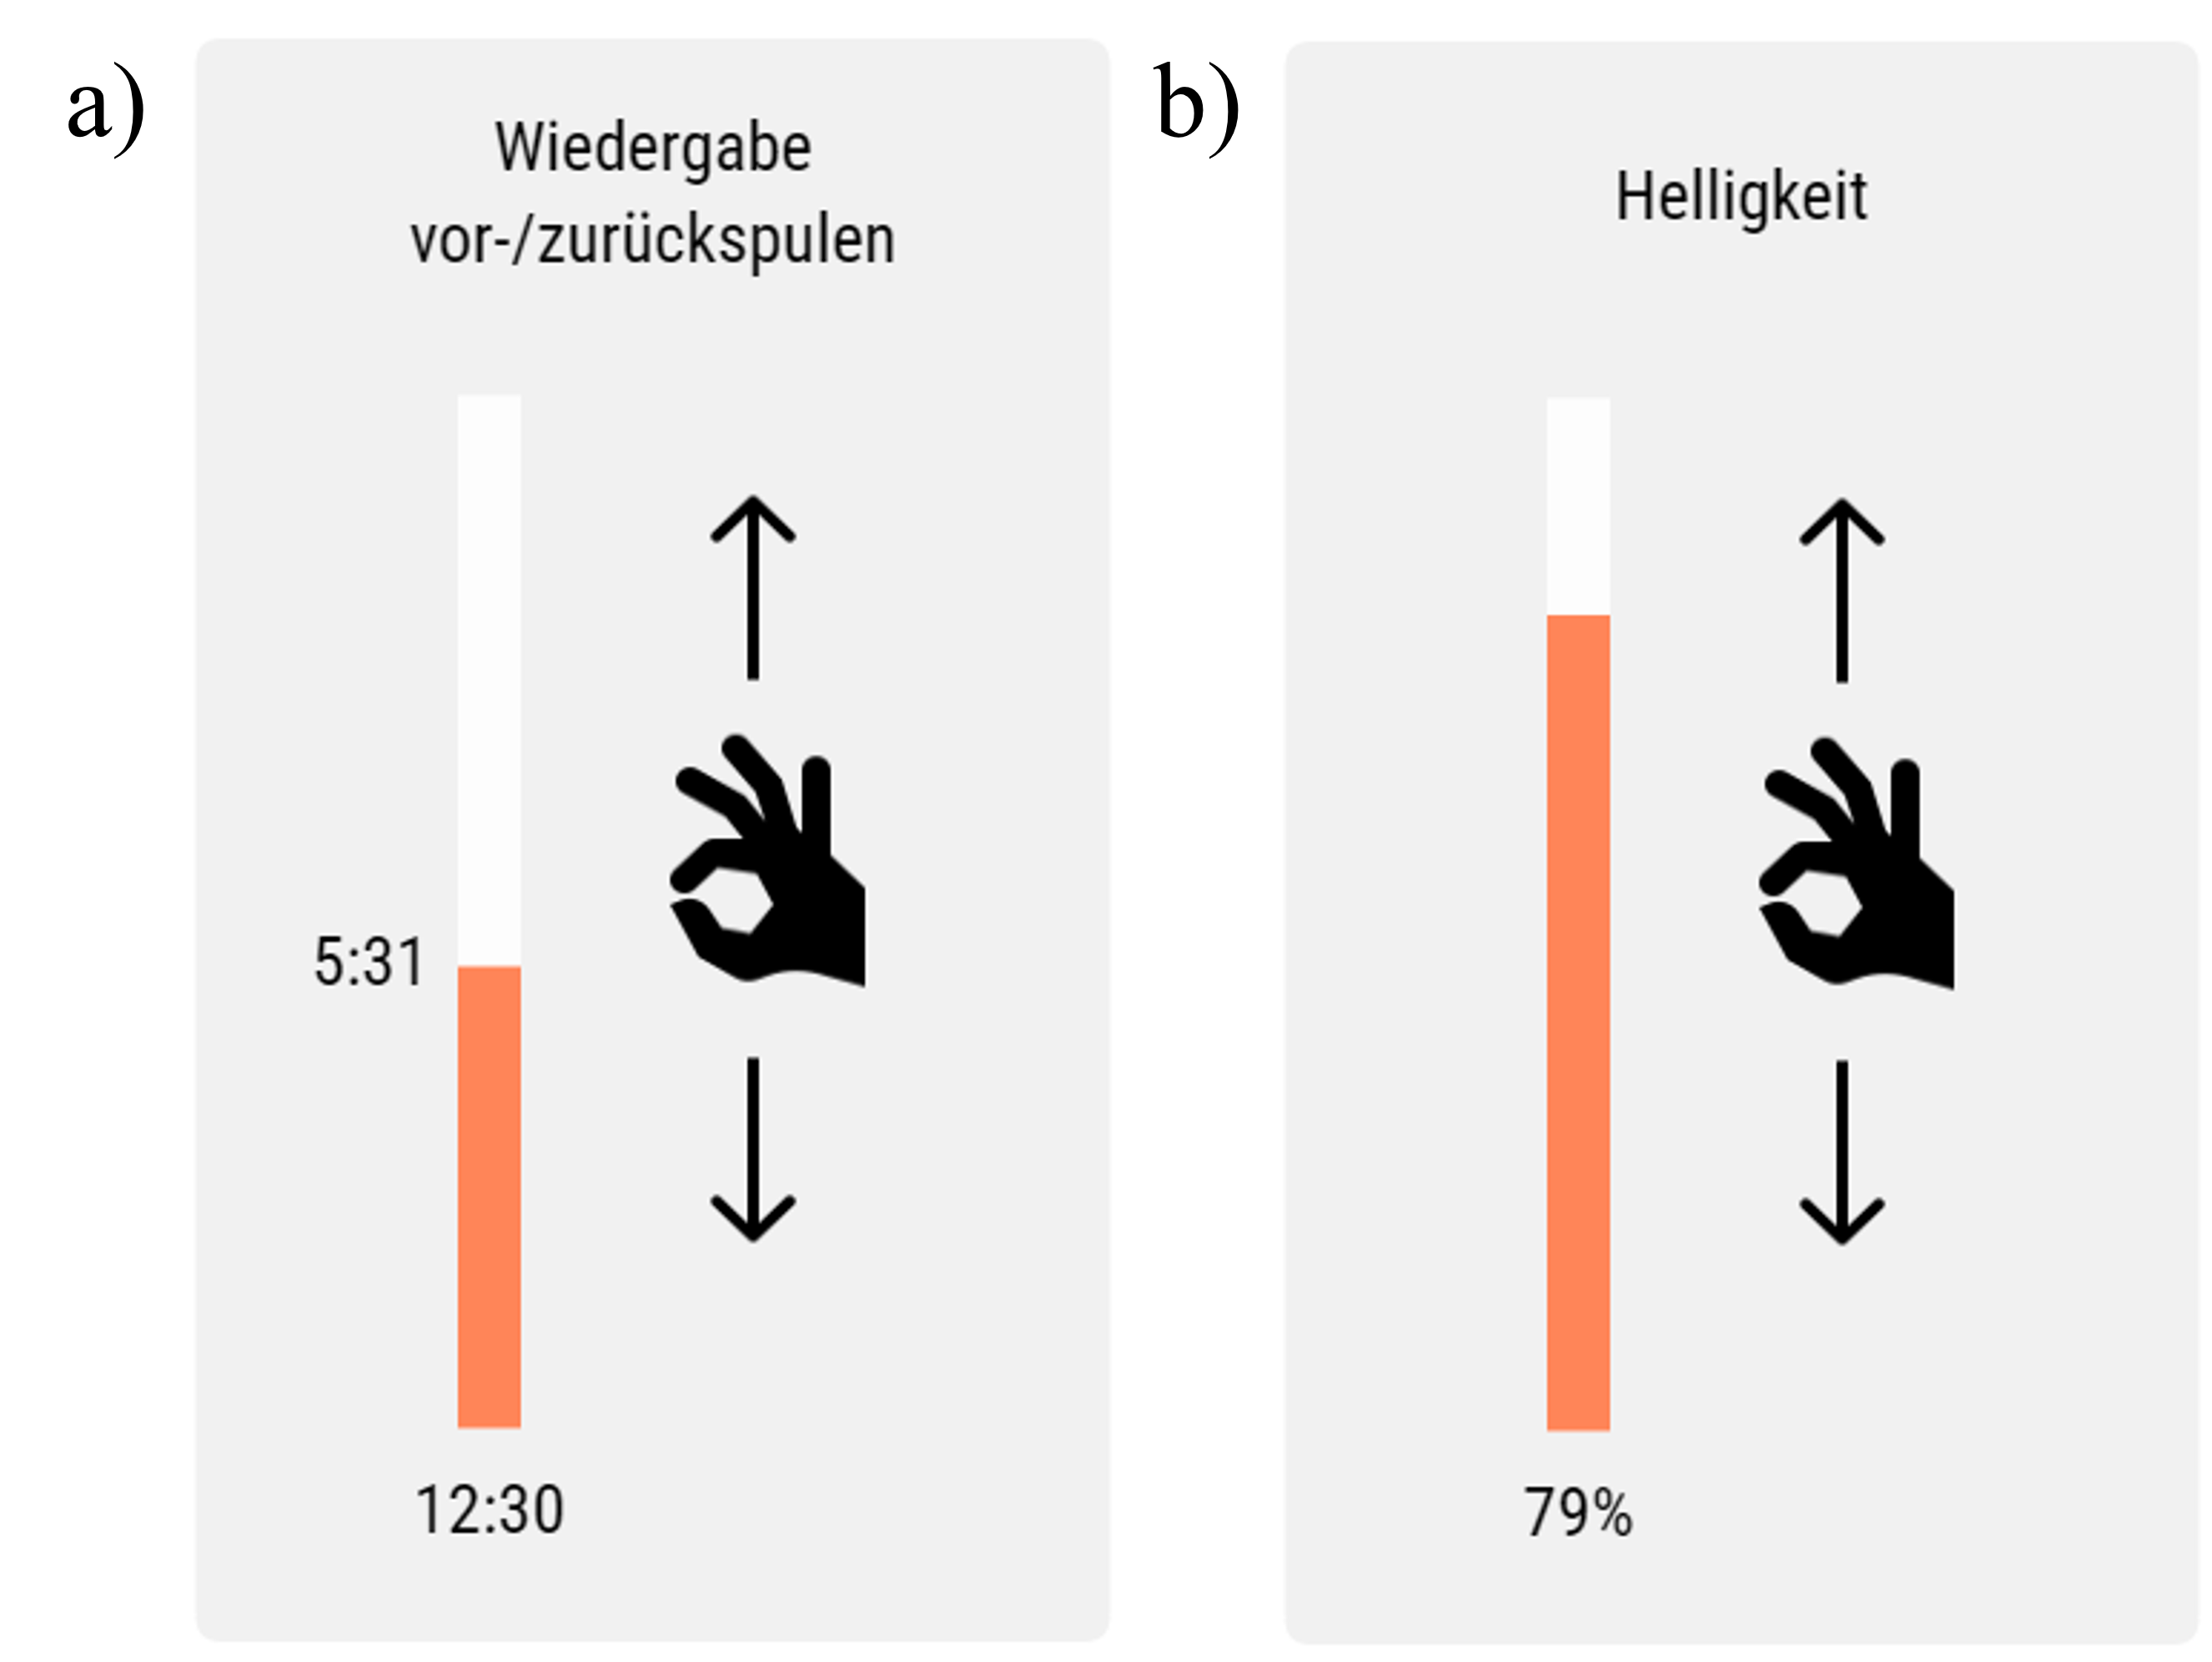
\includegraphics[width=0.5\linewidth]{content/diagrams/Slidertypen.png}
    \caption{Vergleich zweier Slider-Typen: a) zeigt einen zeitbasierten Slider zur Navigation innerhalb eines Videos, b) zeigt einen parameterbasierten Slider mit prozentualer Anzeige. Beide verwenden identische Interaktionsmechanismen bei unterschiedlicher semantischer Bedeutung.}    \label{fig:Slidertypen}
\end{figure}

Ergänzend dazu ist ein Button zur Steuerung der Wiedergabe implementiert, der als klickbares Menüelement realisiert ist. Dieser ermöglicht das Starten und Pausieren von Videomaterial. Der aktuelle Systemzustand wird dabei durch eine visuelle Änderung des Icons kommuniziert, wie in Abbildung \ref{fig:Buttons} dargestellt. Der Button kann wiederholt aktiviert werden und verhält sich funktional analog zu einem klassischen physischen Bedienelement, ist jedoch in die Menüstruktur integriert.

\begin{figure}[H]
    \centering
    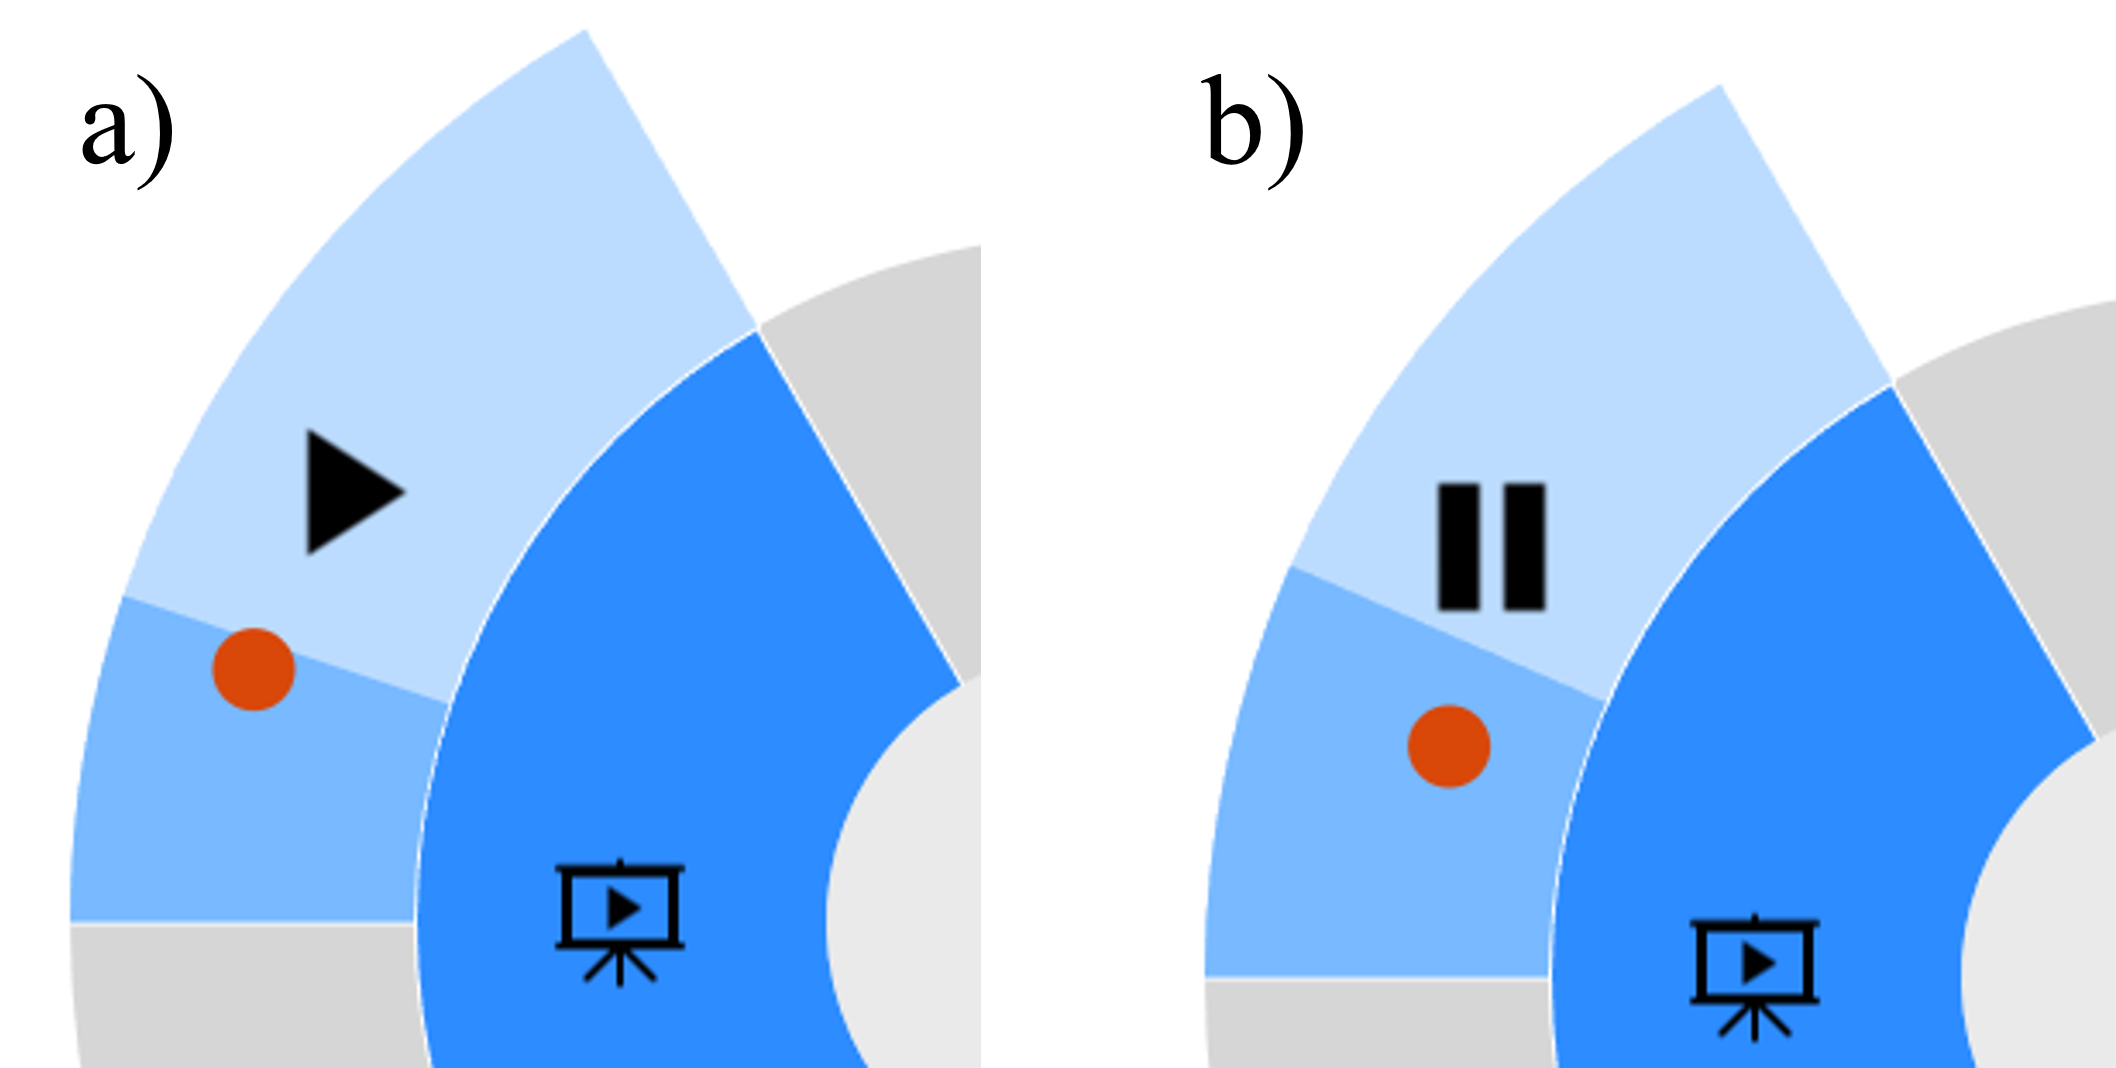
\includegraphics[width=0.5\linewidth]{content/diagrams/Buttons.png}
    \caption{Darstellung der beiden Buttonzustände. a) zeigt den Button, während das Video pausiert ist, b) zeigt den Button, während das Video läuft.}
    \label{fig:Buttons}
\end{figure}

        {\color{red} Muss man für so einen Abschlusssatz ein Zusammenfassungsunterkapitel machen oder ist das ok, wenn das einfach bei Slider mit drin steht? }
% Überagang
Das beschriebene Interaktionskonzept kombiniert somit gestenbasierte Eingaben mit einer strukturierten Menüoberfläche. Durch die Kombination aus radialem Menü, hierarchischen Untermenüs und kontinuierlichen Steuerungselementen können unterschiedliche Interaktionsaufgaben innerhalb eines einheitlichen Systems abgebildet werden. Gleichzeitig bleibt die Interaktion vollständig controllerlos und in den räumlichen Kontext des MIR integriert.
